\chapter{Task-Based Scheduling Solutions}
\label{chapter.scheduling}
In the previous chapter we showed that the most efficient way to utilize an AMC with HPC applications is by performing scheduling in the runtime system level, i.e. using a parallel programmind model.
In this capter our goal is to enhance the current parallel programming models and make them more efficient when it comes to AMCs.

As performance and energy efficiency have become the main challenges for next-generation high-performance computing, asymmetric multi-core architectures can provide solutions to tackle these issues.
Parallel programming models need to be able to suit the needs of such systems and keep on increasing the application's portability and efficiency.
This chapter presents three task scheduling approaches that target asymmetric systems.
These dynamic scheduling policies reduce total execution time either by detecting the longest or the critical path of the dynamic task dependency graph of the application, or by finding the earliest executor of a task.
They use dynamic scheduling and information discoverable during execution, fact that makes them implementable and functional without the need of off-line profiling.
In our evaluation we compare these scheduling approaches against an existing state-of the art heterogeneous scheduler and we track their improvement over a FIFO baseline scheduler.
We show that the heterogeneous schedulers improve the baseline by up to 1.45$\times$ in a real 8-core asymmetric system and up to 2.1$\times$ in a simulated 32-core asymmetric chip.

\newpage

%%%%%%%%%%%%%%%%%%%
%%%%%%%%%%%%%%%%%%%
%Too generig... this should be in the main introduction
%The use of asymmetric multi-core architectures forms an appealing solution in high-performance computing to tackle the power wall.
%These architectures increase energy efficiency~\cite{Fedorova2009,Greenhalgh2011,Casas2015} by featuring different types of processing cores designed to target performance or power optimization.

\section{Introduction}
\label{sec.scheduling.intro}

To effectively utilize AMC systems taking into account their heterogeneity, load balancing and scheduling become two of the main challenges~\cite{Li4}.
An approach towards these challenges is the use of task-based programming models~\cite{OmpSs_PPL11,OpenMP,StarSs,starpu}.
The modern task-based programming models schedule tasks dynamically according to the availability of resources. They also allow the specification of dependencies between tasks, enabling the runtime system to automatically perform scheduling and synchronization decisions.

Even though task-based programming models is a powerful mechanism, the efficient mapping of ready tasks to different types of cores on an asymmetric system remains a challenge when considering the reduction of the total execution time. 
Task-based parallel applications expose different characteristics that can affect the total application duration such as complex task dependency graphs (TDGs) with long critical paths or different levels of task cost variability.
In such cases it is very common that the tasks in the critical path determine the total application duration. 
These characteristics influence researchers to develop smart scheduling techniques within a task-based programming model and accelerate the overall application.
%This opens an opportunity to accelerate the overall application 
The criticality-aware schedulers detect the critical tasks of an application and increase performance by running critical tasks on fast cores. 
Some previous works~\cite{DCPS, LDCP, HEFT, CrPathDup} tackled this issue using static scheduling over the whole TDG to statically map tasks to processors on a heterogeneous system. 
However, they required the knowledge of profiling information and most of them were evaluated on synthetic randomly-generated TDGs. 
%More recent works~\cite{Chronaki:ICS2015} tackle this issue through dynamic task scheduling.

%However, there are no previous works on exploring this possibility in a dynamically scheduled environment.

%There are previous works~\cite{xx} on scheduling of task-based applications onto heterogeneous systems. Their approach is to schedule tasks in the critical path to fast cores but all of them target statically-scheduled applications.

This chapter presents three novel dynamic task schedulers that detect the critical path of the in-flight dynamic snapshot of the TDG. 
Furthermore, this chapter shows the potential of the proposed dynamic scheduling techniques compared to a state-of-the-art dynamic heterogeneous scheduler~\cite{HEFT}.
Specifically we compare our approaches against the a dynamic implementation of the heterogeneous earliest finish time scheduler (HEFT)~\cite{HEFT}.
We implement these scheduling policies in the OmpSs~\cite{OmpSs_PPL11,OmpSs} programming model that supports dynamic scheduling and dependency tracking as described in Section~\ref{sec.background.taskbased}.


%we make a study of the potential of dynamic task scheduling techniques such as the criticality aware task scheduler (CATS)~\cite{Chronaki:ICS2015} and a dynamic implementation of the heterogeneous earliest finish time scheduler (HEFT)~\cite{HEFT} as well as we propose two novel dynamic task schedulers that detect the critical path of the task dependency graph.

%propose a criticality-aware \textit{dynamic} task scheduler that dynamically assigns critical tasks to fast cores to improve performance in a heterogeneous system with fast and slow cores. Compared to previous proposals, this scheduler is based on information discoverable at runtime, is implementable and works without the need of an oracle or profiling. Furthermore, our evaluation is based on a real heterogeneous multi-core platform with real applications and, therefore, using real TDGs.
Compared to previous works, all the scheduling policies described and evaluated in this chapter are based on information discoverable at runtime, are implementable and work on a real asymmetric multi-core platform with real applications and therefore, using real TDGs.
The contributions of this chapter are the following: 
\begin{itemize}
 \item{The Criticality-Aware Task Scheduler (CATS) that dynamically assigns critical tasks to fast cores in an AMC system. Tasks are defined to be critical if they are part of the \textit{longest path} in the in-flight dynamic state of the dependency graph. The flexibility and work stealing policy of this scheduler are configurable. Flexibility increases the number of tasks considered critical. Work stealing may be uni- or bi-directional: only fast cores can steal from slow cores, or slow cores can also steal from fast cores.}
 \item{The Critical Path scheduler (CPATH) that dynamically assigns the tasks that belong to the \textit{critical path} of the TDG to the fast cores of the system. To do so, CPATH tracks the execution time of the tasks, assigns cost-based priorities and, according to these priorities it detects the critical tasks.}
 \item{The Hybrid Criticality scheduler (HYBRID) that incorporates the features of CATS and CPATH by assigning to the fast cores tasks that belong \textit{either to the critical path or to the longest path} of the TDG, depending on the runtime circumstances. HYBRID uses mixed priorities that are cost-based or level-based. This technique also keeps track of the task costs but if this information is not available it uses the mechanisms of CATS that dynamically detects the longest dependency chain of the in-flight dynamic state of the TDG}
 
% Two novel critical path based task schedulers that dynamically assign the tasks that belong to the critical path to the fast cores in a heterogeneous multi-core. First, is the Critical Path scheduler (CPATH scheduler) that keeps track of the task costs and discovers the critical path of the TDG according to these costs. In addition, the Hybrid criticality scheduler (HYBRID) also keeps track of the task costs but if this information is not available it uses the mechanisms of CATS~\cite{Chronaki:ICS2015} that dynamically detects the longest dependency chain of the in-flight dynamic state of the dependency graph.}
 % \item{A novel criticality-aware task scheduler (CATS) that dynamically assigns critical tasks to fast cores in a heterogeneous multi-core. Tasks are defined to be critical if they are part of the longest path in the in-flight dynamic state of the dependency graph. The flexibility and work stealing policy of our scheduler are configurable. Flexibility increases the number of tasks considered critical. Work stealing may be uni- or bi-directional: only fast cores can steal from slow cores, or slow cores can also steal from fast cores.}
 \item{An evaluation of CATS, CPATH and HYBRID schedulers compared to the state of the art heterogeneous scheduler HEFT~\cite{HEFT}, all of them implemented in the OmpSs programming model. Moreover we evaluate these approaches next to the default FIFO scheduler that serves as our baseline.
%We use five scientific benchmarks and we perform our experiments on an Odroid-XU3 development board that features an eight-core Samsung Exynos 5422 chip with ARM big.LITTLE architecture including four Cortex-A15 and four Cortex-A7 cores.
%In addition, our evaluation contains the results on simulated heterogeneous systems that consist of 16 or 32 cores. 
The results show that all heterogeneous schedulers improve overall performance reaching up to 45\% improvement. Furthermore, we describe their features such as the high per-task overheads of CPATH, the inability of dHEFT to improve performance when the task number increases as well as the benefit of HYBRID scheduler compared to CATS when task cost variability increases.
}

% An evaluation of a set of heterogeneous schedulers implemented in the OmpSs programming model and the default OmpSs scheduler. Specifically, we use four heterogeneous schedulers: CATS~\cite{Chronaki:ICS2015}, dHEFT, that is a dynamic implementation of HEFT scheduler~\cite{HEFT}, CPATH, which is the Critical-Path scheduling algorithm proposed in this paper, HYBRID, the second heterogeneous scheduling proposal presented in this paper that uses HYBRID criticality of tasks and BF, which is the default OmpSs scheduler and is used as our baseline. We evaluate the effectiveness of these approaches on different numbers of cores and shares of fast and slow cores on an Odroid-XU3 development board featuring an eight-core Samsung Exynos 5422 chip with ARM big.LITTLE architecture including four Cortex-A15 and four Cortex-A7 cores. We also evaluate the effectiveness of these approaches on larger heterogeneous systems of 16 and 32 cores using simulation. The results show that all heterogeneous schedulers improve overall performance reaching up to 45\% improvement. However we describe their features such as the high per-task overheads of CPATH, the inability of dHEFT to improve performance when the task number increases as well as the benefit of HYBRID scheduler compared to CATS when task cost variability increases.}
 
 %The results show that CATS constantly improves overall performance reaching up to 38\% improvement over the baseline. Moreover, dHEFT also improves the baseline by up to 45\% but the results show that by increasing the number of tasks, the performance of dHEFT decreases. The CPATH scheduler, struggles to improve the baseline by up to 23\% due to the increased per task overheads during the critical path exploration process. Finally, HYBRID 
 
% and in some cases HYBRID scheduler outperforms CATS showing improvement of 17\%. On the other hand, CPATH scheduler suffers }

% \item{An evaluation of our implementation of CATS in the OmpSs programming model compared to a dynamic implementation of Heterogeneous Earliest Finish Time \cite{HEFT} and the default OmpSs scheduler. We evaluate the effectiveness of CATS on different numbers of cores and shares of fast and slow cores on an Odroid-XU3 development board featuring an eight-core Samsung Exynos 5422 chip with ARM big.LITTLE architecture including four Cortex-A15 and four Cortex-A7 cores. We also evaluate the effectiveness of CATS on different speed ratios between fast and slow cores using simulation of heterogeneous multi-cores with up to 128 cores. The results show that CATS improves overall performance up to 1.3$\times$ on the real eight-core platform, and up to 2.7$\times$ on a simulated 128-core~system.}
\end{itemize}
Table~\ref{tab.acronyms} shows the acronyms that we use in the next sections.
% We describe a set of configurations for our scheduler regarding the work stealing capabilities of the different core types and the flexibility to define a task as critical or non-critical. 
 
% We implement this scheduler in OmpSs and evaluate its effectiveness on different numbers of cores and shares of fast and slow cores on a real system. 
 
% We also evaluate the effectiveness of our scheduler depending on the speed ratio between fast and slow cores using simulation.  The results show that the effectiveness of our scheduler increases with larger numbers of fast cores over slow cores, and with larger differences of performance between fast and slow cores.

%Finally, we provide a set of recommendations on how to configure our scheduler to get the best results depending on the target system size and configuration.
\begin{table}
\begin{center}
\caption{Acronyms used in the paper \kc{Move all acronyms at the beginning of the thesis? Or remove them totally?}}
\label{tab.acronyms}
\begin{tabular}{|c|c|}
\hline
 \textbf{Acronym} & \textbf{Meaning}\\\hline\hline
TDG & Task Dependency Graph \\
CATS & Criticality-Aware Task Scheduler\\
CPATH & Critical Path-Aware Scheduler\\
HEFT & Heterogeneous Earliest Finish Time\\
dHEFT & Dynamic Heterogeneous Earliest Finish Time\\
BF & Breadth-First\\
HYBRID & Hybrid Criticality-Aware Scheduler\\
FIFO & First-In First-Out\\
\texttt{plist} & Predecessors' List\\
\texttt{slist} & Successors' List\\
tt-is & Task Type - Input Size\\
\hline
\end{tabular} 
\end{center}
\vspace{-0.4cm}
\end{table}

%%%%%%%%%%%%%%%%%%%
%%%%%%%%%%%%%%%%%%%
%\section{Heterogeneous Scheduling}
%\label{sec:scheduling}
The efficient scheduling problem has been intensively studied for asymmetric systems.
In this section we describe four scheduling approaches that target such systems.
The first three are based on separating the tasks into groups of critical and non-critical tasks and assign each group to one core type: the critical tasks to the fast cores and the non-critical tasks to the slow cores.
The difference between these three approaches is the way of considering a task critical.
First is the Criticality-Aware scheduler (CATS)\cite{Chronaki:ICS2015}, which detects the critical tasks based on their \textit{bottom level}.
Secondly, the Critical Path scheduler (CPATH), proposed in this paper, that detects the critical path of the dynamic (TDG) with the help of \textit{bottom cost} based priorities.
The Hybrid Criticality scheduler (HYBRID), proposed in this paper, uses both bottom level and bottom cost based priorities.
Last, we describe a dynamic implementation of HEFT scheduler (dHEFT)~\cite{HEFT}, that for every task it detects the processor that finishes its execution at the earliest possible time.
All of the described schedulers operate at runtime on the dynamic snapshots of the TDG. 
CPATH, HYBRID and dHEFT perform on-line profiling of the task execution time without considering inter-task communication costs, given the uncertainty of data movement latency that hides in the cache hierarchy of an asymmetric multi-core system with prefetching. 
%but none of these schedulers track the inter-task communication costs.


\lstset{basicstyle=\footnotesize\ttfamily,
        emphstyle=\bfseries,
        columns=fixed,
        numbers=none,
        moredelim=*[l][\textit]{//},
        moredelim=*[l][\bfseries]{\#},
        literate={...}{\dots}3
} 
\subsection{Criticality-Aware Task Scheduler}
\label{sec.cats}
The Criticality-Aware Task Scheduling generally applies to task-based programming models supporting task dependencies, but for simplicity we explain it in the context of the OmpSs programming model.
CATS uses bottom-level longest-path priorities and consists of three steps:
%\begin{itemize}

\textbf{Task prioritization}: when a task is created and added to the TDG, it is assigned a priority and the priority of the rest of tasks in the graph is updated accordingly.
 %Since the task graph is generated at runtime, there is no way to statically compute the priority that will be given to a task. 

\textbf{Task submission}: when a task becomes \textit{ready}, i.e., all its predecessors finished their execution, it is submitted to a \textit{ready queue}. At this point, the algorithm decides whether the task is considered \textit{critical} or \textit{non critical}. The task is then inserted in the corresponding ready queue: tasks in the \textit{critical ready queue} will be executed by fast cores, and tasks in the \textit{non-critical ready queue} will be executed by slow cores.

\textbf{Task-to-core assignment}: when a core becomes idle, it tries to retrieve a task from its corresponding ready queue to execute it. If the queue is empty, it might try to steal from the other queue according on the work stealing policy. %Currently, we support two work stealing mechanisms: \textit{simple} work stealing, i.e., fast cores can steal from slow cores; and \textit{bidirectional} (\textit{2DS}) work stealing, i.e., both types can steal from the other. The default policy is \textit{simple}.
%\end{itemize}

These steps are performed dynamically and potentially in parallel in different cores. Thus, while some tasks are being prioritized, previously created tasks may be submitted, and others assigned to available cores or executed.

To give an overview of the scheduling process, Figure~\ref{botlevels} shows a scheme of the operation of CATS. In the TDG on the left, each node represents a task and each edge of the graph represents a dependency between two tasks. The number inside each node is the \textit{bottom level} of the task: the length of the longest path in the dependency chains from this node to a leaf node. The priority of a task is given by its bottom level. The pattern-filled nodes indicate tasks that are considered critical. The number outside each node is the task id and is used in the text to refer to each task. Critical tasks are inserted in the critical queue, and non-critical tasks to the non-critical queue. The insertion is ordered with the highest priorities at the head of the queue and the lowest priorities at the tail. Slow cores retrieve tasks from the head of the non-critical queue and fast cores from the critical queue. The following sections describe these scheduling steps in~detail.


\begin{figure}[t]
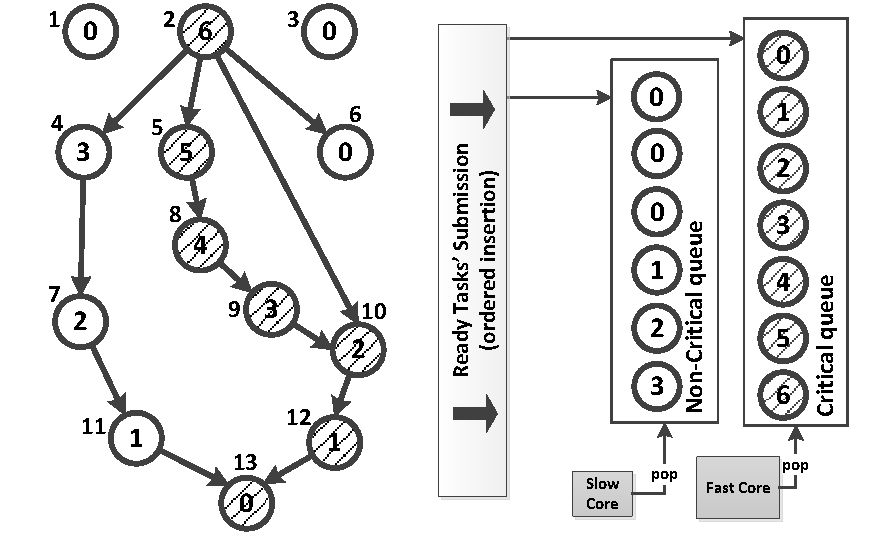
\includegraphics[width=\columnwidth]{images/fig_1.pdf} 
\centering
\caption{Task submission with CATS. Nodes are marked with the \textit{bottom level} of each task. Pattern-filled nodes mark the critical tasks.}
\label{botlevels}
\vspace{-0.5cm}
\end{figure}


\subsubsection{Task Prioritization}

Each task in the TDG has a list to include its predecessors (\textit{plist}). Every time an edge is added into the TDG on the creation of a new task, the corresponding predecessor of the dependency is added in the \textit{plist} of its successor. For example, in Figure~\ref{botlevels}, when the dependency between tasks~2 and~5 occurs, the task number~2 is inserted into the \textit{plist} of the task number~5. Thus, the \textit{plist} of task number~5 becomes $\{$2$\}$. Accordingly, the \textit{plist} of task number~10 will be $\{$2, 9$\}$ when the edge~9$\rightarrow$10 is inserted to the TDG. 

%Right after the occurrence of a dependency between two tasks, the task prioritization step takes place, once for each edge of the graph. 
%represented by the edges in the graph, that connect one predecessor task with one successor task.

The priority given to a task is the \textit{bottom level} of the task. The \textit{bottom level} is computed by traversing the TDG upwards starting from the successor that the currently created edge is pointing to. The priority of this successor is 0 because it is a leaf node of the graph, as it is the last created task. Then, using \textit{plist} for each task, the algorithm navigates to the upper levels of the TDG and updates the priority on each visited node. This way not all the graph is updated, but only the tasks that are predecessors in the paths to the new edge. The algorithm also stops going up through a path, when it finds a priority larger than the one it would be updated to.

Listing~\ref{creation} shows the algorithm for task prioritization. The complexity of this is \textit{O($n^2$)}, \textit{$n$} being the number of tasks. This function is called on the creation of a new edge with the successor as argument. The algorithm traverses the \textit{plist} of the successor task (line 5) and if the priority of the current predecessor is lower than the bottom level of the successor plus one, it updates the current predecessor's priority to that value (lines 7-8). If the updated predecessor task is ready (i.e., it sits in one of the ready queues), the scheduler reorders the ready queue so it remains ordered considering the updated priority (lines 9-10). Then, the same actions are performed recursively for each predecessor of the \textit{plist} to update all the possible upward paths from the successor. 

The terminate conditions for the TDG navigation are two: \textit{(a)} if the \textit{plist} of the current task (\texttt{currPred}) is empty, so either we reach an entry node or the predecessors of the task have finished execution; or \textit{(b)} if the priority of the current task (\texttt{currPred}) remains unchanged, which means that the successor task (\texttt{succ}) does not belong to the longest path because its predecessor already has a higher priority. 
\begin{lstlisting}[float, emph={void,if,return,non_critical_queue, critical_queue,prioritize_task}, captionpos=b, caption={Pseudo-code task prioritization with CATS.},label=creation, emph={[2]mat}, emphstyle={[2]}, aboveskip={0\baselineskip}, frame=tb, belowskip={-0.4cm}]
1 void prioritize_task(task *succ) {
2  int blev = succ->priority;
3  list plist = plistOf(succ);
4  task *currPred;
5  while( not isEmpty(plist) ) {
6    currPred = plist.next();  
7    if(priorityOf(currPred) < blev+1) {
8     currPred->priority = blev+1;
9     if(isReady(currPred)) 
10     readyQueueOf(currPred)->reorder();
11    prioritize_task(currPred);
12   }
13 }
14}
\end{lstlisting}
\subsubsection{Task Submission}

%CATS supports two task submission policies: the \textit{flexible} policy adds more task in the critical queue for the fast cores, while the \textit{strict} policy reduces the number of critical tasks.

The purpose of this step is to divide the tasks into two groups: \textit{critical} and \textit{non-critical}. Critical tasks are tasks that belong to the longest path of the dynamic TDG, namely the path  with the maximum number of tasks (or nodes). Thus, the longest path starts from the task with the maximum bottom level. At runtime, the longest path changes as tasks complete execution and new tasks are created. CATS manages to detect these changes and dynamically decide if the submitted task belongs to the longest path of the TDG.

When a task's dependencies are satisfied, the task becomes ready for execution and is to be inserted in the \textit{ready queues}. Ready queues are priority queues that keep tasks in a decreasing order of task priorities, i.e., the task with the maximum priority resides on the head of the queue. Critical tasks are inserted in the critical queue and non-critical tasks in the non-critical queue. The pattern-filled nodes in Figure~\ref{botlevels} represent the critical tasks in that graph. 

%This way, tasks in the critical queue will then be scheduled to fast cores, and non-critical tasks to slow cores.

%By keeping track of the last discovered critical task%task with the maximum priority
To determine the criticality of a task, CATS keeps track of the last discovered critical task. Then, for each task that becomes ready, CATS checks the following conditions:
%, our approach to detect critical tasks in the graph is to check the following two conditions for each task that becomes ready:
\textit{(a)} if the priority of the current ready task is higher or equal to the priority of the last discovered critical task and, \textit{(b)} if the current ready task is the highest-priority immediate successor of the last discovered critical task.

%%%%%%%%%%%%%%%%%%%%%%%%%%%%%%%%%%%%%%%%
\if 0 %flexible strict explanation
In the first case, the algorithm detects new longest paths that may have been created by the application throughout the execution of a prior longest path. In this case, the scheduler can either be \textit{strict} or \textit{flexible}:
\begin{itemize}
 \item{\textit{Strict}: marks as critical tasks with priority higher than the priority of the last critical task.}
 \item{\textit{Flexible}: marks as critical tasks with priority higher or equal to the priority of the last critical task.} 
 \end{itemize}
As a result, the flexible scheduler ends up with more critical tasks than the strict. The flexibility of the scheduler can be set by the programmer through an environment variable.
\fi % about flexible/strict explanation
%%%%%%%%%%%%%%%%%%%%%%%%%%%%%%%%%%%%%%%%%%%%
\begin{figure}[tl!]
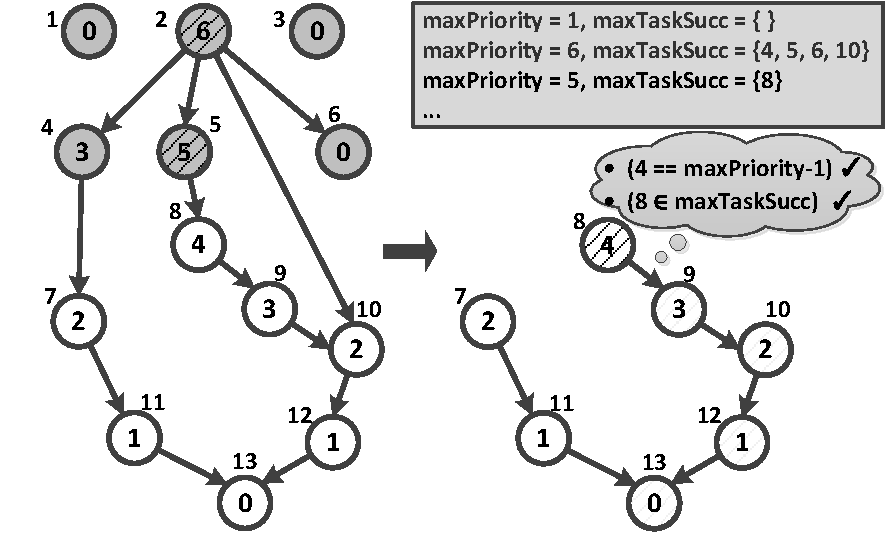
\includegraphics[width=\columnwidth]{images/fig_2.pdf} 
\centering
\caption{Task submission. Gray nodes indicate finished tasks and pattern-filled nodes indicate critical tasks.}
\label{submitFig}
\vspace{-0.5cm}
\end{figure}
The task that satisfies the second condition is a task with a lower priority than the maximum but the task belongs to the longest path because it is the highest priority immediate successor of the last detected critical task. 

Listing~\ref{submission} shows a simplified version of the task submission code, that is of complexity \textit{O($n$)} (\textit{$n$} is the number of tasks). The variable \texttt{maxPriority} (line 1) is used to store the priority of the last critical task, and \texttt{maxPriorityTask} (line 2) is used to store the last critical task. Initially, \texttt{maxPriority} is set to 1 and \texttt{maxPriorityTask} is set to \texttt{NULL}. This avoids the scheduling of independent tasks (i.e., tasks with zero priority) to fast processors at the start of the execution. On the first ready task, if its priority is higher or equal than 1 (line 5) , it is considered to be the first task of the longest path. Therefore, it is inserted in the critical queue and the variables \texttt{maxPriority} and \texttt{maxPriorityTask} are updated accordingly (lines 9-11) to determine correctly the criticality of the next submitted task.

If the priority of the submitted task is equal to \texttt{maxPriority - 1}, we check if it also belongs to the successors of the task with the maximum priority (lines 6-7) and therefore to the longest path. If these two conditions are met, the task is determined to be critical, it is inserted in the critical queue and, as before, the variables \texttt{maxPriority} and \texttt{maxPriorityTask} are updated (lines 9-11). In the rest of the cases the task is not considered critical and it is inserted in the non-critical queue.

Figure~\ref{submitFig} shows an example of a TDG during task submission. The gray nodes in the graph are tasks that have finished execution and the pattern-filled nodes are critical tasks. The numbers inside the nodes indicate their priority and the numbers outside the nodes show the task id, which is assigned in task creation order. The variable \texttt{maxPriority} corresponds to the priority of the last critical task and the \texttt{maxTaskSucc} is the list of the successors of the last critical task, filled with the task ids of the successors. Initially, \texttt{maxPriority} is set to~1 and \texttt{maxTaskSucc} is empty. When task~2 is about to be submitted, it is inserted in the critical queue because its priority is higher than the maximum, which at the beginning is~1. Then, the value of \texttt{maxPriority} is set to~6 (priority of task~2), and the \texttt{maxTaskSucc} list is updated with the successors of task~2. At the point where all the gray tasks have finished execution, the values of \texttt{maxPriority} and \texttt{maxTaskSucc} are updated as shown  in Figure~\ref{submitFig}. For every newly-ready task, the conditions listed above are evaluated. When task~7 is submitted, it is not considered as critical because it does not belong to the \texttt{maxTaskSucc} list and its priority is not equal to \texttt{maxPriority-1}. Contrarily, task 8 satisfies both conditions and so the task is inserted in the critical queue.

\begin{lstlisting}[float, emph={void,if,return,non_critical_queue, critical_queue,submit_task}, captionpos=b, caption={Pseudo-code for task submission with CATS.},label=submission, emph={[2]mat}, emphstyle={[2]}, aboveskip={0\baselineskip}, frame=tb, belowskip={-0.4cm}]
1 int maxPriority = 1;
2 task *maxPriorityTask = NULL;
3
4 void submit_task(task *t) {
5  if( t->priority >= maxPriority or
6     (t->priority == maxPriority-1 and
7      t $\in$ succListOf(maxPriorityTask)) )
8  { //the task is critical
9    critical_queue.push(t);
10   maxPriority = priorityOf(t);
11   maxPriorityTask = t;
12   return;
13 }
14 //the task is non-critical
15 non_critical_queue.push(t);     
16}
\end{lstlisting}

\subsubsection{Task-to-Core Assignment}
\label{sec.cats.assignment}
Task-to-core assignment takes place dynamically and in parallel to the previous steps and its time complexity is \textit{O($n$)}, \textit{$n$} being the number of tasks. When a core becomes idle, it checks the corresponding ready queue (depending on the core type) to get a task to execute. Fast cores retrieve critical tasks from the critical queue, while slow cores retrieve non-critical tasks from the non-critical queue. Each ready queue is shared among the cores of the same type so there is no need for work stealing among cores of the same type. 

If tasks in an application are imbalanced, i.e., the majority are non-critical and only a few tasks are critical, or vice versa, one of the types of processors would be overloaded and the other would starve for work. This can happen in applications with wide graphs and a large amount of tasks, where the ratio between critical tasks and the total amount of tasks may be small. To leverage the resources, the work-stealing mechanism for CATS lets fast cores steal work from slow cores whenever the critical queue becomes empty. 
%Also, CATS can be configured to perform \textit{bidirectional work stealing} so slow processors can also steal tasks from the critical queue if the non-critical queue is empty. 
%We evaluate these different options and show the results in the next section.

\section{Critical Path Scheduler}
\label{sec.scheduling.cpath}
\begin{figure}[tr]
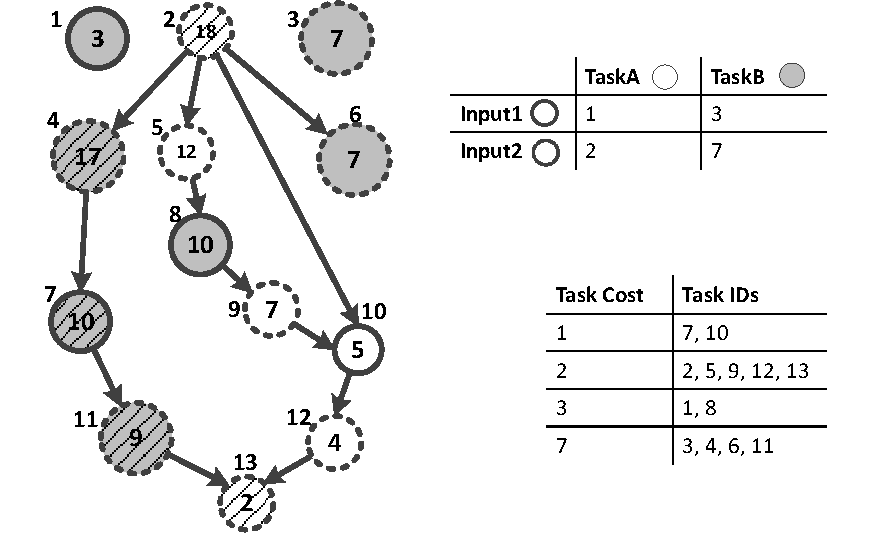
\includegraphics[width=\columnwidth]{images/cpath_priorities.pdf} 
\centering
\caption{Priority assignment taking into account the task costs. Task costs are assumed known and are shown in the tables.}
\label{cpath}
\vspace{-0.5cm}
\end{figure}


The Critical Path scheduler (CPATH) dynamically detects the critical path of the TDG.
Like CATS, CPATH separates tasks into two groups: critical and non-critical tasks.
The detected critical tasks are executed by the fast cores in the system and non-critical tasks are executed by slow cores.
The difference with CATS is the algorithm for critical path detection.
CPATH takes into account the task execution time, about which CATS is unaware.
To do so, CPATH implements a more complex and accurate critical path detection algorithm that takes into account task execution time.

CPATH scheduler consists of three steps:
%\begin{itemize}

\textbf{Task prioritization}: this step takes place when a task is finishing its execution. This is different than CATS since at the end of a task execution the algorithm may record the task execution time (task cost).
%might track a new (unknown) task cost. 
According to the discovered task cost CPATH assigns priorities to tasks by traversing the TDG from top to bottom, introducing the cost of \textit{O($2n^2$)}, where \textit{$n$} is the number of tasks.

\textbf{Task submission}: when a task becomes \textit{ready}, it is submitted to a \textit{ready queue}. At this point, CPATH decides whether or not the task is \textit{critical} and inserts it in the corresponding ready queue. This step has only slight implementation differences with CATS and complexity of \textit{O($n$)}.

\textbf{Task-to-core assignment}: this step is identical to CATS.
% and supports the same work stealing mechanisms.

%\end{itemize}

\subsection{Task Prioritization}
%explanation of the slist (successors' list)

Each task of the TDG keeps a list with its successors (\textit{slist}).
This list is being built when an edge (dependency between two tasks) is added in the TDG.
So when a task dependency occurs, the corresponding successor task is added in the \textit{slist} of its predecessor.
For example, on Figure~\ref{cpath}, when the dependency between tasks 2 and 4 occurs, the \textit{slist} of task number 2 becomes \{4\}. 
This goes on for all the added edges of the TDG, therefore when the edge~2$\rightarrow$5 is inserted in the TDG, the task number 5 is inserted in the \textit{slist} of task number 2; so the \textit{slist} of task number 2 becomes \{4, 5\}.

The goal of this step is to assign priorities based on the \textit{bottom cost} of the tasks of the TDG.
We define the \textit{bottom cost} of a node on a directed acyclic graph as the maximum estimated time in the dependency chains from this node to a leaf node.
So the main difference between the \textit{bottom level} and the \textit{bottom cost} is the consideration of the estimated time.

Figure~\ref{cpath} is used to describe the priority assignment with CPATH.
The specific TDG contains tasks of two different types and two different input sizes.
Node color shows the different task types and the outline of the circle (dashed or solid) shows the different input sizes.
The upper table in Figure~\ref{cpath} indicates the execution time of the tasks according to their type and input size.
The algorithm assumes that task instances of the same type with the same input size have the same (or very similar) execution time.
To track this information, CPATH discovers the cost of every possible task type-input size duple (tt-is duple) that appears on the TDG.
The numbers inside the nodes show the bottom cost-based priorities that CPATH assigns and the numbers outside the nodes show their task ID.


%This task type-input size duple is denoted as tt-is and the algorithm assumes that the task with the same tt-is have the same execution time.
%So the execution time of the tasks differs according to the task type-input size duple (\texttt{tt-is} duple).
%CPATH discovers the cost for all the tt-is pairs and prioritizes the tasks according to their \textit{bottom cost} as shown on Figure~\ref{cpath}.
%The bottom cost of a node is equal to the maximum estimated time in the dependency chains from this node to a leaf node.

The task prioritization step takes place every time a task finishes execution. 
CPATH uses a vector to store task costs and keeps one entry per tt-is.
Because CPATH needs to discover the unbiased critical path of the TDG, it uses one of the core types as reference to track the task costs.
%So at the beginning of the execution tasks are executed on one of the core types during this cost-learning phase.
In our experiments we chose to use as reference the fast cores since this way the learning phase (that is, the phase where CPATH discovers the task costs) becomes shorter.
To avoid wrong task cost prediction of future tasks, CPATH ignores the first execution of each tt-is because usually it takes more time. 
\begin{lstlisting}[float, emph={for,in,void,if,return,updatePriorities,non_critical_queue, critical_queue,submit_task}, captionpos=b, caption={Pseudo-code for taskExit, the function called by the cores used as reference for tracking the task costs},label=cpathExit, emph={[2]mat}, emphstyle={[2]}, aboveskip={0\baselineskip}, frame=tb, belowskip={-0.4cm}]
1 void taskExit (task* finished) {
2  if( stateOf(finished) == init ) {
3    finished->state = in_progress;
4    return;
5  }
6  if( stateOf(finished) == in_progress ) {
7    timesSet[finished] = finished->execTime;
8    finished->state = tracked;
9  }
10 task* succ;
11 for( succ in finished->successors ) 
12   if( numPredecessorsOf(succ) == 1 ) {
13     lock();
14     if( succ $\notin$ entryNodes ) 
15       entryNodes->push(succ);
16       unlock();
17   }
18 list<task>* updatedList = new list<task>();
19 for( node in entryNodes) 
20   updatePriorities(node, updatedList);
21 for( node in updatedList ) 
22    node->unsetUpdated();
23}
\end{lstlisting}

Listings \ref{cpathExit} and \ref{cpathUpdate} show how the critical path scheduler performs task prioritization.
Whenever a task finishes execution on one of the cores used as reference (here: fast cores) the runtime makes a call to the \texttt{taskExit} routine shown in Listing~\ref{cpathExit}.
At this point, the runtime is aware of the execution time of the finished task.
This function has the responsibility to update the known task costs and also perform the prioritization of the tasks on the TDG.
The prioritization is done by the \texttt{updatePriorities} function of Listing~\ref{cpathUpdate}. 
This function is responsible for TDG traversal.

The \texttt{taskExit} function in Listing~\ref{cpathExit} takes as an argument the task that has just finished. 
In order to keep track of whether the execution time of the tt-is has been discovered we implement a small finite state machine within this stage.
Every tt-is has three possible states. 
The initial state is the \texttt{init} state; this means that the specific tt-is has not yet been executed so its execution time is totally unknown.
When a tt-is is executed for the first time its state changes from \texttt{init} to 
\texttt{in$\_$progress}. 
This means that a task of this tt-is has been executed once, but CPATH ignores this cost because the first instance may not be representative due to cold start effects and one sample may not be enough history for prediction.
While the tt-is of a node is in \texttt{init} or \texttt{in$\_$progress} state its execution time is considered to be 1.
%we have to ignore this execution because usually it takes too long and is not representative.
After the second execution of a tt-is the state of it becomes \texttt{tracked} meaning that the execution time has been tracked and can be used for the computation of the priorities.
%If the node does not have a known execution cost tracked, we consider its execution time to be 1.

After the first checks of the tt-is state (lines 2-9 of Listing~\ref{cpathExit}) the algorithm traverses the \textit{slist} of the finished task and searches for the successors that become ready by the end of the execution of this task.
This is identified by the fact that the ready-to-be successors have one unique (remaining) predecessor (e.g. the just finished task).
These successors are inserted in the \texttt{entryNodes} list (lines 11-16 of Listing~\ref{cpathExit}).
For each one of the entry nodes the \texttt{updatePriorities} function is called (line 19 of Listing~\ref{cpathExit}); this performs a top to bottom traversal of the TDG and updates the priorities.

\begin{lstlisting}[float, emph={for,in,void,if,return,non_critical_queue, critical_queue,submit_task}, captionpos=b, caption={Pseudo-code for task prioritization with CPATH},label=cpathUpdate, emph={[2]mat}, emphstyle={[2]}, aboveskip={0\baselineskip}, frame=tb, belowskip={-0.5cm}]
1 int updatePriorities (task* currT, list* updated) {
2   if( currT == NULL )  return 0;
3   if( isVisited(currT) )  
4     return priorityOf(currT);
5   successors = currT->successors;
6   int maxSucc = -1;
7   bool succVisited = true;
8  
9   for(succ in successors) {
10    int succPriority;
11    //Avoid double update
12    if( !isUpdated(succ) || !isVisited(succ) ) {
13      succPriority = updatePriorities(succ, updated);
14      succ->setUpdated();
15      updated->push(succ);
16    }
17    else 
18      succPriority = priorityOf(succ);
19    if(succPriority > maxSucc)
20       maxSucc = succPriority;
21    succVisited = succVisited && isVisited(succ);   
22  }
23  if( timeIsTracked(currT) ) {
24    currT->priority = (maxSucc + timesSet[currT]);
25    if(succVisited && groupOf(currT) < twDetected) 
26      currT->setVisited();
27  }  
28  else
29    currT->priority = maxSucc + 1;
30    
31  return priorityOf(currT);  
32}
\end{lstlisting}

Due to the properties of the top-to-bottom TDG traversal, the algorithm has to make sure that every node is prioritized only once per \texttt{updatePriorities} call.
This is controlled by checking the \texttt{updated} flag of each node of the TDG.
To visualize this situation let us assume that task number 2 of the TDG on Figure~\ref{cpath} finishes.
Then the \texttt{entryNodes} list contains three tasks that will start the update: \{4, 5, 6\}.
The update that starts from task number 4 marks tasks 4, 7, 11 and 13 as updated.
Then, during the update of task number 5, the algorithm knows that task 13 has already been prioritized during the same update so there is no need to apply the algorithm at this node again.
This example does not show too much optimization because in this case the update of only one node is saved, but in real applications this node could have numerous successors for whom the priority update would be a large overhead.

The raising of the \texttt{updated} flag is something temporal and is only used for helping the prioritization of a single update.
There are cases when CPATH needs to raise a permanent flag in order to mark that the priority of the task will not change again in the future, e.g. it is the final priority.
This happens when the execution times of all the tt-is that appear on the TDG have been discovered, for the tasks that their priorities are up to date.
To mark these tasks CPATH uses the \texttt{visited} flag.
If a task is \texttt{visited}, there is no need to get prioritized again.
To clarify this, let us assume that in Figure~\ref{cpath} the task costs of the tt-is TaskA-Input2 and TaskB-Input2 are known.
During the next prioritization, tasks 11 (TaskB-Input2), 12 (TaskA-Input2) and 13 (TaskA-Input2) in the TDG will be set as visited, because their priorities consist of the sum of known task execution times and they do not have any successors (with unknown execution times).
So, an additional priority update in cases like this is redundant.
%So, the algorithm does not need to visit these nodes again on the current update, nor on a future priority update.


%Moreover, CPATH prioritization needs to make sure that the priority of a to-be-updated node is not the final priority.
%In case that the priority of a node is final then there is no need for updating this node.
%To perform this check, CPATH checks the \texttt{visited} flag of every node, which tells if the priority of the node is final.
%To understand what a final priority is, let's assume that CPATH has discovered the task costs of the tt-is TaskA-Input2 and TaskB-Input2 on the Figure~\ref{cpath}.
%This means that the tasks 11, 12 and 13 of the TDG are visited, because their priorities are not going to change since they consist of the sum of known task execution times and they don't have any successors.
%So, the algorithm does not need to visit these nodes again not on the current update, neither on a future priority update.



%For example, in Figure~\ref{cpath}


%Because one node might get updated more than once through different possible paths, we optimize the procedure by keeping the \texttt{updated} flag. 
%This flag tells whether the node has been updated during the prioritization that caused the exit of the same task. 
%This way duplicate updates on a single task exit are skipped and we make sure that the nodes are updated only once.
%At the end of this routine the updated flag is being unset because the nodes have to be updated in case a new task cost is discovered in a future task exit.

Listing~\ref{cpathUpdate} shows what happens during the the update of one entry node.
The arguments of this function are \texttt{currT}, that is the entry node being updated, and \texttt{updated}, that is the list with the updated nodes. 
This list is being filled throughout the priority update in order to unset the updated flag later.
The lines 2-4 of Listing~\ref{cpathUpdate} perform the checks that would cause the traversal to finish.
If the node is not visited, then the algorithm traverses its successors.
Note that, at this point, there is no check for updated flag, since tasks in the \texttt{entryNodes} are unlikely to be updated. 
Updated nodes can only be discovered through recursive calls and this check is performed later.
%this cannot happen from the entryNodes, only from recursive calls which is checked later.
If a successor is updated or visited, the priority update is skipped for the reasons explained above. 
Otherwise, the \texttt{updatePriorities} is called recursively for the current successor.
This happens until we detect a node that is updated, visited or is a leaf node (node with no successors) of the TDG.
When the algorithm reaches a node ready for update it calculates its priority by summing the highest priority of its successors to the execution time, if known, of the current node (lines 24, 29).
Finally, the visited flag of the task is being updated. 

There are three conditions that mark a task as visited: \textit{(a)} if its execution time is known (line 23),  \textit{(b)} if \textbf{all} of its successors are visited (line 25) or \textit{(c)} if we have encountered a taskwait (barrier) after the creation of this task (line 25).
%To mark a node as visited we have to check the following:
%\begin{itemize}
%\item If the execution time tracked of this tt-is is known (line 23)
%\item If \textbf{all} of the task's successors are visited (line 25)
%\item If we have encountered a taskwait (barrier) after the creation of this task (line 25)
%\end{itemize}
%In addition to the updated flag, the algorithm uses the \texttt{visited} flag.
%The algorithm is not using only the updated flag to mark the updates; each node in the TDG can be marked as \texttt{visited} as well.
%The \texttt{visited} flag tells to the algorithm that the node has a valid and unchangeable priority.
%This shows that the priorities of all the descendants of this task have valid execution times tracked and their priorities are computed according to these final values. 
%Thus there is no need to traverse the successors of a visited node and this is an important optimization of the algorithm.
%
%As described, the lines 2-4 of Listing~\ref{cpathUpdate} perform the checks that would cause the traversal to finish.
%If the node is not visited, then the algorithm traverses its successors.
%If a successor is updated or visited the update of priorities is skipped. 
%Otherwise, the \texttt{updatePriorities} is called recursively using the current successor as an entry node.
%This happens until we find a node that has been updated or is visited or a leaf node (node with no successors) of the TDG.
%When the algorithm reaches a node ready for update it calculates its priority by summing the highest priority of its successors with the execution time, if known, of the current node (lines 24, 29).
%If the node does not have a known execution cost tracked, we consider its execution time to be 1.
%Finally, the visited flag of the updated task is being updated. 
%To mark a node as visited we have to check the following:
%\begin{itemize}
%\item If the execution time tracked of this tt-is is valid
%\item If \textbf{all} of the task's successors are visited
%\item If we have encountered a taskwait after the creation of this task
%\end{itemize}
The last condition confirms that it is safe to mark this task as visited as there will be no future successors of this task on the current TDG. 
%The reason behind the last condition is that if we have encountered a taskwait \textbf{after} the creation of this task this means that there will be no future successors on the current TDG. 
%Thus, we do not need to worry about setting priorities on tasks that reside below the visited tasks of the TDG.
To track this information we use an atomic variable, \texttt{twDetected}, which is increased every time a taskwait is encountered.
At creation time, each task is assigned a group ID which is the value of the \texttt{twDetected} at that moment.
%This way the tasks are separated into groups according to the detected taskwaits.
%At creation time, tasks are separated into groups according to the detected taskwaits by assigning as group ID the value of the \texttt{twDetected} at that moment.
If the group ID of a task is less than the current \texttt{twDetected} value then this means that a taskwait has occurred after the creation of this task.

\subsection{Task Submission} 
The task submission is implemented using the same \texttt{critical} and \texttt{non-critical} ready queues as in CATS.
Listing~\ref{submission} can be used to describe the task submission of CPATH.
The only modification needed is in the condition of the lines 6 and 7 of Listing~\ref{submission}.
In addition to the \texttt{maxPriority}, CPATH keeps track of the \texttt{maxExecTime} which is the cost of the last discovered critical task.
CPATH extends the condition of the critical task consideration by checking whether the priority of the current task is equal to \texttt{maxPriority} - \texttt{1} or if it is equal to \texttt{maxPriority} - \texttt{maxExecTime}.
Moreover, the value of \texttt{maxExecTime} is updated accordingly to the \texttt{maxPriority}.

\subsection{Task-to-Core Assignment}
Task-to-core assignment in CPATH is identical to CATS as described in Section~\ref{sec.cats.assignment}. 
It takes place dynamically and in parallel to the previous steps.
Depending on the core type, whenever a core becomes idle it retrieves a task from its corresponding ready queue; fast cores are responsible for the execution of the tasks in the critical queue and slow cores for the tasks in the non-critical queue.
Each ready queue is shared among the cores of the same type so there is no need for work stealing among cores of the same type. 
Finally, as with CATS, the work-stealing mechanism prevents load imbalance by allowing big cores to steal work from the little cores.






\section{Hybrid Criticality Scheduler}
\label{sec.scheduling.hybrid}

The Hybrid Criticality Scheduler (HYBRID) is a combination of the CATS and CPATH scheduling policies.
HYBRID keeps the simplicity of the implementation of CATS and introduces the task execution time only if available.
This results in an efficient low-overhead scheduler that computes the critical path of a TDG more faithfully than CATS and with lower overheads than CPATH.
%The idea for this is again based on separating the critical and non-critical tasks and execute the critical tasks on the fast cores of the system.
This section describes HYBRID through its relation to CATS and CPATH described in Sections~\ref{sec.cats} and~\ref{sec.cpath}. 
We focus our description on the task prioritization, since task submission and task-to-core assignment for HYBRID are identical to CPATH.

As shown, CPATH computes priorities on task completion. 
The algorithm for priority computation is an expensive operation and is in the critical path of the execution:
on task completion the core becomes available but the start of the next task is delayed by priority computation.
Also, when multiple cores are completing tasks, there will be contention on accessing the TDG for priority computation.
On the other hand, CATS computes priorities during task creation.
The computation of priorities during task creation is more efficient because, unless there is nested parallelism, one core creates all tasks
and therefore there is no contention on priority computation. The downside is that there is potentially less information available 
on tt-is pair execution time on task creation, as some task type may have not been executed yet at the time all tasks are created.
%there is only one core involved in this procedure responsible for the creation of the tasks.
%In addition, the rest of the cores are exclusively used for executing tasks undisturbed.

%, where it is more unlikely to have information about the task execution time. 

%In an effort to reduce the scheduling overheads of CPATH, we implement HYBRID. 
HYBRID tracks task execution time on task completion and stores this information in a vector.
This means that it also implements the \texttt{taskExit} function of CPATH that is called on task completion but, in the case of HYBRID, \texttt{taskExit} is only responsible of recording the execution time of the exiting task.
This functionality is represented in lines 2-9 of Listing~\ref{cpathExit} and, after this code, the function returns.
% in HYBRID takes place during task creation because as described above this reduces the scheduling overheads.
The priority assignment, taking place on task creation, remains similar to CATS \footnote{All of the HYBRID scheduling steps have the same time complexity as CATS} with the only difference that task cost is used for priority computation only if known and, otherwise, the cost is assigned to 1 and priority is increased according to CATS (lines 7 and 8 of Listing~\ref{creation}).

%high-level differences:
%% This could be simplified, also given there is a short mention before
When comparing CPATH and HYBRID schedulers their logical operation is similar.
However the difference in their implementation may result in different task priorities potentially leading to different schedules.
For applications with small TDGs, HYBRID may not be able to compute an accurate critical path because task creation does not overlap with a sufficient amount of task exits.
%Therefore, priority computation will not have enough information about task execution time and HYBRID will prioritize based on bottom-level priorities (like CATS).
Therefore, task execution information will not be available during priority computation and HYBRID will prioritize based on bottom-level priorities (like CATS).
If the application has a large TDG and task creation overlaps with a sufficient amount of task exits, HYBRID will use bottom-cost priorities.
%CPATH on the other hand, updates priorities right after task cost is known, which leads to a more faithful critical path computation. 

\begin{figure}[tr]
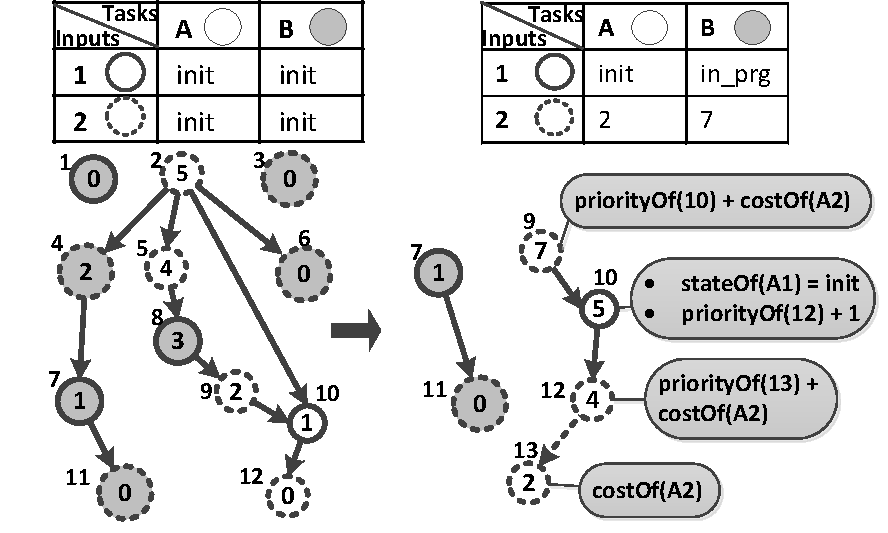
\includegraphics[width=\columnwidth]{images/hybrid_prioritization.pdf} 
\centering
\caption{Priority assignment with HYBRID scheduler. Priority update when the edge between tasks 12 and 13 is created}
\label{hybrid_priorities}
\vspace{-0.5cm}
\end{figure} 

Figure~\ref{hybrid_priorities} shows an example of task prioritization with HYBRID.
The tables show the state (or exec. time) of the tt-is pairs that appear on the TDG. Gray or white nodes indicate different task types (A or B respectively) and solid or dashed node outlines indicate task input size (1 or 2 respectively). The numbers inside the nodes show task priorities and the numbers outside the nodes show the task id.

On the leftmost TDG, the algorithm has no information about any of the tt-is costs.
As the leftmost table shows, for all the possible tt-is the state is \texttt{init} meaning no task has been executed yet.
Since the tasks of the TDG have been created, they have been prioritized using the CATS priority assignment method and the bottom level based priorities.
On the rightmost TDG, tasks 1, 2, 3, 4, 5, 6 and 8 have been executed and a new task has appeared on the TDG: task number 13.
When the edge 12$\rightarrow$13 is created, tasks begin to be prioritized.
Initially, the priority of the new task 13 is the cost of this task's tt-is, i.e., type A and input 2 (TaskA-Input2). 
Since there are no successors of this task, this becomes its initial priority.
Then, the \textit{plist} of task 13 is traversed and the priority of task 12 changes to priorityOf(13)+costOf(TaskA-Input2) since task 12 is corresponding to the TaskA-Input2 tt-is.
Moving to the upper levels, task 10 is of tt-is TaskA-Input1 that is on the \texttt{init} state, thus unknown cost.
This translates to the use of bottom level based prioritization so the priority of task 10 becomes priorityOf(12)+1.
Finally, task 9 is prioritized using the cost of the TaskA-Input2 tt-is and the TDG navigation stops since there are no other predecessors.

\if 0


Like CPATH, HYBRID prioritizes tasks according to their \textit{bottom cost} and/or their \textit{bottom level}.

HYBRID constitutes of three steps: \textit{Task Prioritization, Task Submission} and \textit{Task-to-core assignment.}


\subsubsection{Task prioritization}
The HYBRID scheduler prioritizes tasks according to their \textit{bottom cost} and/or their \textit{bottom level}.
The task prioritization step takes place during task creation.
%If when a dependency is created the execution time of the tt-is of the successor is known, then it is used for the prioritization.
If task cost information is available, HYBRID uses it to compute priorities.
Otherwise, the algorithm computes priorities the same way as CATS, that is, increasing the priority as we move to higher levels of the TDG.

%task execution time tracking:
As tasks are being executed HYBRID collects their execution times.
A vector is used to store the execution time of every tt-is discovered throughout the execution.
When a task finishes execution, HYBRID calls the \texttt{taskExit} function.
This function is responsible for tracking the execution time of the exiting task by storing it in the vector.
As in CPATH, \texttt{taskExit} ignores the first execution of every tt-is.
Therefore, the functionality of a small finite state machine is needed for each tt-is.
To start with, a tt-is is in the \texttt{init} state; when the tt-is has been executed once its state changes from \texttt{init} to \texttt{in$\_$progress} to skip the cost of the first execution.
After the second execution of the same tt-is, \texttt{taskExit} stores its execution time in the vector and its state becomes \texttt{tracked}.
This functionality is represented in the lines 2-9 of Listing~\ref{cpathExit}.
After this code, the function returns, since HYBRID does not perform any prioritization when a task is finishing execution.

The task prioritization step takes place when a new task is added to the TDG.
%Because the addition of a new task on the TDG always takes place at the (one) bottom of the graph, the use of the \textit{plist} (list of predecessors) of the tasks, is essential in order to perform a bottom-to-top TDG traversal.
HYBRID uses the \textit{plist} (list of predecessors as used in CATS) of the new task to navigate to the upper levels of the TDG and update the task priorities.

Listing~\ref{creation} shows the algorithm of the task prioritization with CATS.
Because HYBRID uses a very similar algorithm we will describe it using the same code while highlighting the differences.
When a new task is created, if its tt-is execution time is known, it is assigned as the priority of the new task. 
If there is no cost information the priority assigned to the new task is initially zero.
The \texttt{prioritize$\_$task} function is called on the creation of a new edge on the TDG between two tasks: the predecessor task and successor task.
It takes as argument the successor task and starts by traversing its \textit{plist} (line 5).
The HYBRID algorithm then checks whether the predecessor task has a tracked execution cost.
If so, it checks whether the priority of the current predecessor is lower than the priority of the successor plus the cost of the predecessor and, if this condition is met, the priority of the predecessor is updated accordingly.
In the case that the cost of the predecessor has not been tracked, the algorithm checks if the priority of the current predecessor is lower than the priority of the successor plus one (as on line 7 of Listing~\ref{creation}).
In the first case, HYBRID scheduler uses bottom cost based priorities, like CPATH, while in the latter case, it uses bottom level based priorities, like CATS.
In both cases, if the priority of the predecessor has changed and the predecessor task is a ready task (i.e. it sits on one of the ready queues) the corresponding ready queue is being reordered considering the updated priority (lines 9-10).

The same actions are performed for the predecessors of the upper levels of the TDG.
The algorithm, similarly to CATS, terminates if it encounters an empty \textit{plist} or if the priority of the current predecessor task (\texttt{currPred}) remains unchanged.


Figure~\ref{hybrid_priorities} shows an example of task prioritization with HYBRID.
The tables show the state (or the exec. time) of the tt-is pairs that appear on the TDG.
Gray or white nodes indicate different task types (type A or B respectively) and solid or dashed node outlines indicate the task input size (input 1 or 2 respectively).
The numbers inside the nodes show task priorities and the numbers outside the nodes show the task id.

On the left-most TDG the algorithm has no information about any of the tt-is costs.
As the left-most table shows, for all the possible tt-is the state is \texttt{init} meaning no task has been executed yet.
Since the tasks of the TDG have been created, they have been prioritized using the CATS priority assignment method and the bottom level based priorities.
On the right-most TDG tasks 1, 2, 3, 4, 5, 6 and 8 have been executed and a new task has appeared on the TDG: task number 13.
When the edge 12$\rightarrow$13 is created, tasks begin to get prioritized.
Initially, the priority of the new task 13 is the cost of this task's tt-is which is of type A and input 2 (A2). 
Since there are no successors of this task this becomes its initial priority.
Then, the \textit{plist} of task 13 is traversed and the priority of task 12 changes to the priorityOf(13)+costOf(A2) since task 12 is corresponding to the A2 tt-is.
Moving to the upper levels, task 10 is of tt-is A1 that is on the \texttt{init} state, thus unknown cost.
This translates to the use of bottom level based prioritization so the priority of task 10 becomes priorityOf(12)+1.
Finally, task 9 is prioritized using the cost of the A2 tt-is and the TDG navigation stops since there are no other predecessors.
\fi

\if 0
It then checks whether the priority of the current predecessor is greater than the priority of the successor





If the cost of a tt-is of a task is known at the time of the task's creation then this cost is used as priority to the task that is being created.
If the cost of the tt-is is unknown then the priority of the new task becomes \texttt{1}.

The result that we try to achieve in terms of priorities is the same as in Figure~\ref{cpath}. 
First, we need to track the task execution times.
HYBRID implements a simplified version of the function \texttt{taskExit} for doing so. 
The \texttt{taskExit} in HYBRID scheduler is responsible for tracking the execution time of each task-type/input size (tt-is) and store it to the time vector.
To simplify our description, the code of the HYBRID \texttt{taskExit} contains the lines 1-9 of Listing~\ref{cpathExit}.
While task costs are being tracked, other tasks are being prioritized.
The task prioritization step is similar to CATS shown in Listing~\ref{creation} featuring a minor difference. 
In the lines 7 and 8 of Listing~\ref{creation} HYBRID scheduler checks whether the cost of the current tt-is has been discovered; if it has been discovered, it increases the priority (\texttt{blev} in the code) by this cost, otherwise it increases the priority by 1.
This way, the tasks end up being prioritized with the bottom-cost-based priority as in the case of CPATH but only if the tt-is cost has been discovered.

%In this case this function simply checks if the execution time for the current task-type/input-size duple has been tracked.
%If not then we update the execution time of the timesSet with the elapsed time of the finished task.
%Meanwhile we use the \texttt{task$\_$prioritization} function; in this case, instead of always increasing the bottom-level by 1, the task$\_$prioritization querries the timesSet to find out whether the execution time has been computed.
%If we have a valid execution time, then the bottom level of the predecessor is increased by this value instead of 1.
\subsubsection{Task Submission and Task-to-Core Assignment}
The task submission and task-to-core assignment steps are identical to CPATH.


%For the task submission step we slightly modify the submit$\_$task function.
%In this case the scheduler has to keep track of the execution time of the last discovered critical task.
%By keeping this information available in the scheduler we can then decide if a successor belongs to the critical path by subtracting the maxExecution time instead of subtracting 1.
%Even if the execution time of the last discovered critical task is not known this returns a correct result because in case the execution time has not been tracked the lookup function returns 1 so automatically the bottom-level-based priority is taken into account.
%\subsubsection{Task-to-core assignment}
%This step is identical to the one of CATS.

The hybrid scheduler tries to compute the critical path in the most efficient way.
The critical path computation is approximate since the priorities on the TDG are not updated as soon as in the case of CPATH.
However even if the priorities do not take into account the execution time, the HYBRID manages to use the properties of CATS to perform well.
\kc{Maybe remove this sentence?:}
We expect that this scheduler will perform better if the input TDG features tasks that differ in execution time as well as if the TDG features a great number of tasks (e.g. thousands) so that their execution time is discovered before the end of their execution.

\fi

\subsection{Dynamic Heterogeneous Earliest Finish Time Scheduler}
The Heterogeneous Earliest Finish Time (HEFT) algorithm~\cite{HEFT} is a static scheduling approach for asymmetric systems.
HEFT consists of two compile-time phases that use profiling information: the \textit{task prioritizing phase} and the \textit{processor selection phase}.
In the first phase, the algorithm assigns priorities to the tasks based on their \textit{upward rank}, that is, the length of the critical path from a given task to the exit task including task computation and communication costs~\cite{HEFT}.
When task prioritizing is done, the tasks are sorted according to their priorities.
In the \textit{processor selection phase} the algorithm searches for each task the appropriate processor to execute it.
By keeping communication and computation costs, HEFT assigns each task to the processor that will finish its execution at the earliest possible time.
Topcuoglu et al. \cite{HEFT} present their results based on evaluation on synthetic TDGs and assume known task execution and communication times at compile time.
The scheduling is static, so all the decisions are taken before execution.

In this paper, since the evaluation consists of running real applications with unknown task costs, the best way to compare HEFT to our proposal is by using a dynamic version of HEFT algorithm (dHEFT).
The dHEFT is implemented in the OmpSs programming model and is based on the implementation used in the evaluation of CATS~\cite{Chronaki:ICS2015}.
This version assumes two different types of cores (fast and slow) and keeps records of the task costs in each core.
DHEFT discovers the task costs at runtime, computes the mean cost of each tt-is for each core type and then finds the core that will finish the task at the earliest possible time.

To find the earliest possible executor, dHEFT maintains
one list per core (wlist) including the ready tasks waiting
to be executed by that core. 
When a task becomes ready, dHEFT first inserts it in the ordered ready queue; then the task with the highest upward rank is selected and dHEFT checks if there are execution time records for this task. 
If the number of records is sufficient (we require a minimum of three records)
then the estimated cost of the task is considered stable. 
Using that estimated execution time, the task
is scheduled to the earliest executor by consulting the wlist
of all cores. If the number of records is not sufficient
for one of the core types, then the task is scheduled to the
earliest executor of this core type to get another record of
that task-type and core-type execution time. In all cases,
dHEFT updates the history of records on every task execution to adapt for phase changes in the application. \footnote{The time complexity of the task submission step is \textit{O($nN$)} and the task-to-core assignment is \textit{O($n$)}, where \textit{$n$} is the number of tasks and \textit{$N$} is the number of cores.}

The initial dHEFT version presented in previous work~\cite{Chronaki:ICS2015} lacks the \textit{task prioritizing phase} of the original HEFT algorithm.
This paper, uses an improved version of dHEFT that adds this functionality by prioritizing tasks according to their \textit{upward rank}.
The implementation of this is similar to the CPATH prioritization step.
%to the tasks whenever an undiscovered tt-is has finished its execution.
%The TDG is traversed from the top to the bottom and, using task execution times, the upward-rank-based priorities are assigned to tasks.
When the prioritized tasks become ready, they are inserted in a sorted ready queue in decreasing order of their priorities.
The algorithm then accesses the tasks in the order of their priorities to find the earliest executor for each of them.


%%%%%%%%%%%%%%%%%%%
%%%%%%%%%%%%%%%%%%%
%\section{Experimental Methodology}
%\label{sec:experimental}
%\begin{table*}[t]
\begin{center}
\caption{Evaluated benchmarks and relevant characteristics}
\label{tab.apps}
\resizebox{\textwidth}{!}{%
\begin{tabular}{|c|c|c|c|c|c|c|c|c|c|}
\hline
\multirow{3}{*}{\parbox{13mm}{\centering Application}} & 
\multirow{3}{*}{Problem size} & 
\multirow{3}{*}{\parbox{10mm}{\centering \#Tasks}} & 
\multirow{3}{*}{\parbox{17mm}{\centering Avg task CPU cycles (thousands)}} & 
\multicolumn{3}{|c|}{\parbox{22mm}{\centering Per task overheads (CPU cycles)}} & & &\\
\cline{5-7}
& & & & \multirow{2}{*}{\parbox{10mm}{\centering Create}} & \multirow{2}{*}{\parbox{9mm}{\centering All}} & \multirow{2}{*}{\parbox{11mm}{\centering Deps + Sched}} & \multirow{2}{*}{\parbox{15mm}{\centering Measured perf. ratio}} &
{\parbox{10mm}{\centering $r$}} &
\multirow{2}{*}{\parbox{11mm}{\centering Parallel model}} \\
& & & & & & & & & \\ %\hhline{~~~~~~}
\hline

\multirow{2}{*}{\parbox{18mm}{\centering Cholesky factorization}} & 
32K 256 & 357\,762  & 753 & 15221 &  73286 &  58065 &  \multirow{2}{*}{\parbox{9mm}{\centering 3.5}} & 10.34 & \multirow{2}{*}{\parbox{17mm}{\centering dependencies}}\\                                              & 32K 128 & 2829058 & 110 & 17992 &  58820 &  40828 & & 83.74 &\\
%& 32$\times$32 blocks of 512$\times$512 floats & 5984 & & 1\,551\,322 & 104.76 &  238.02 &  194.28  & \\ 
\hline{}
\multirow{2}{*}{\parbox{18mm}{\centering QR factorization}} & 16K 512 & 11\,442 & 518\,570  & 17595 & 63008 &   45413 & \multirow{2}{*}{\parbox{9mm}{\centering 6.8}} & 0.01 &\multirow{2}{*}{\parbox{17mm}{\centering dependencies}}\\
&  16K 128 & 707\,265 & 3\,558 & 21642 & 60777 & 39135 & & 3.11 &\\
\hline
Blackscholes & native & 488\,202 & 348  &   29141  &  85438 &  56297 & 2.3 & 42.87 & data-parallel \\
\hline
Bodytrack & native & 329\,123 & 383 &  9\,505 &  18979 & 9474 & 4.2 & 12.70 & pipeline \\ 
%Heat diffusion & Heat &  &  &  &  &  & \\ 
\hline
Canneal & native & 3\,072\,002 & 67 & 25781 & 50094 &  24313 & 2.0 & 197.01 & unstructured \\
\hline
Dedup & native & 20\,248 & 1\,532 & 1294 & 9647 &  8353 & 2.7 & 0.43 & pipeline \\
\hline 
Ferret & native$\times$2 & 84\,002 & 29\,088 & 38913 & 98457 &  59544 & 3.6 & 0.68 & pipeline \\
\hline
Fluidanimate & native & 128\,502 & 16\,734 & 30210 & 94079 &  64079 & 3.3 & 0.91 & data-parallel \\
\hline
Streamcluster & native & 3\,184\,654 & 161 & 6892 & 13693 &  6801 & 3.5 & 21.91 & data-parallel \\
\hline
\end{tabular}}
\end{center}
\vspace{-0.4cm}
\end{table*}

\subsection{Applications}
%\begin{itemize}
%\item Blackscholes
%\item Cholesky
%\item Canneal
%\item Fluidanimate
%\item QR Factorization
%\item Bodytrack
%\item Streamcluster
%\end{itemize}
Table~\ref{tab.apps} shows the evaluated applications, the input sizes used, and their characteristics. 
All applications are implemented using the OpenMP programming model~\cite{OpenMP4.0:Manual2015}. 
We obtain Cholesky and QR from the BAR repository~\cite{BAR} and we use the implementations of the rest of the benchmarks from the PARSECSs suite~\cite{Chasapis:TACO2016}.
More information about these applications can be found in~\cite{Chasapis:TACO2016} and~\cite{Chronaki:ICS2015}.
As the number of cores in SoCs is increasing, so does the need of available task parallelism~\cite{Sanchez:2010}. 
We choose the input sizes of the applications so that they create enough fine-grained tasks to feed up to 512 cores.
The number of tasks per application and input as well as the average per-task CPU cycles can be found on Table~\ref{tab.apps}.





\subsection{Simulation}
\label{TaskGenX:experimental:simulation}
To evaluate TaskGenX we make use of the TaskSim trace-driven simulator~\cite{AbstrLevels_TACO12,MUSA} as explained in Section~\ref{sec.background.simulation}. 

We evaluate both symmetric and asymmetric systes with the number of cores varying from 8 to 512.
To set the correct performance ratio between big and little cores for the asymetric systems, we measure the sequential execution time of each application on a real ARM big.LITTLE platform when running on a little and on a big core. 
We use the Hardkernel Odroid~XU3 board that includes a Samsung Exynos 5422 chip with ARM big.LITTLE.
The big cores run at 1.6GHz and the little cores at 800MHz.
Table~\ref{tab.apps} shows the measured performance ratio for each case.
The average performance ratio among our 11 workloads is 3.8.
Thus in the specification of the asymmetric systems we use as performance ratio the value 4.

We modify TaskSim so that it features one extra hardware accelerator (per multi-core) responsible for the fast task creation (the RTopt).
Apart from the task duration time, our modified simulator tracks the duration of the runtime overheads.
These overheads include: (a) task creation, (b) dependencies resolution, and (c) scheduling.
The RTopt core is optimized to execute task creation faster than the general purpose cores; 
to determine how much faster a task creation job is executed we use the analysis performed in Section~\ref{sec:hw_req}.

Using Equation~\ref{eq.create}, we compute the $C_{opt}(x)$ for each application according to their average task CPU cycles from Table~\ref{tab.apps} for $x=512$ cores.
$C_{gp}$ is the cost of task creation when it is performed on a general purpose core, namely the \textit{Create} column shown on Table~\ref{tab.apps}.
To have optimal results for each application on systems up to 512 cores, $C_{gp}$ needs to be reduced to $C_{opt}(512)$.
Thus the specialized hardware accelerator needs to perform task creation with a ratio $r = C_{gp}/C_{opt}(512) \times$ faster than a general purpose core.

We compute $r$ for each application shown on Table~\ref{tab.apps}. We observe that for the applications with a large number of per-task CPU cycles and relatively small \textit{Create} cycles (QR512, Dedup, Ferret, Fluidanimate), $r$ is very close to zero, meaning that the task creation cost ($C_{gp}$) is already small enough for optimal task creation without the need of a faster hardware accelerator.
For the rest of the applications, more powerful hardware is needed.
For these applications $r$ ranges from 3$\times$ to 197$\times$.
Comparing $r$ to the measured performance ratio of each application we can see that in most cases accelerating the task creation on a big core would not be sufficient for achieving higher task creation rate.
In our experimental evaluation we accelerate task creation in the RTopt and we use the ratio of 16$\times$ which is a relatively small value within this range that we consider realistic to implement in hardware.
%Contrarily, if RTopt is assigned a task to execute, we assume that it executes it 4$\times$ slower than a general purpose in-order core.
The results obtained show the average results among three different traces for each application-input.

%%%%%%%%%%%%%%%%%%%
%%%%%%%%%%%%%%%%%%%
\section{Evaluation}
\label{sec.scheduling.evaluation}


\subsection{Methodology}
\begin{figure}[t]
	\centering
	\subfloat[Cholesky 8$\times$8]{
		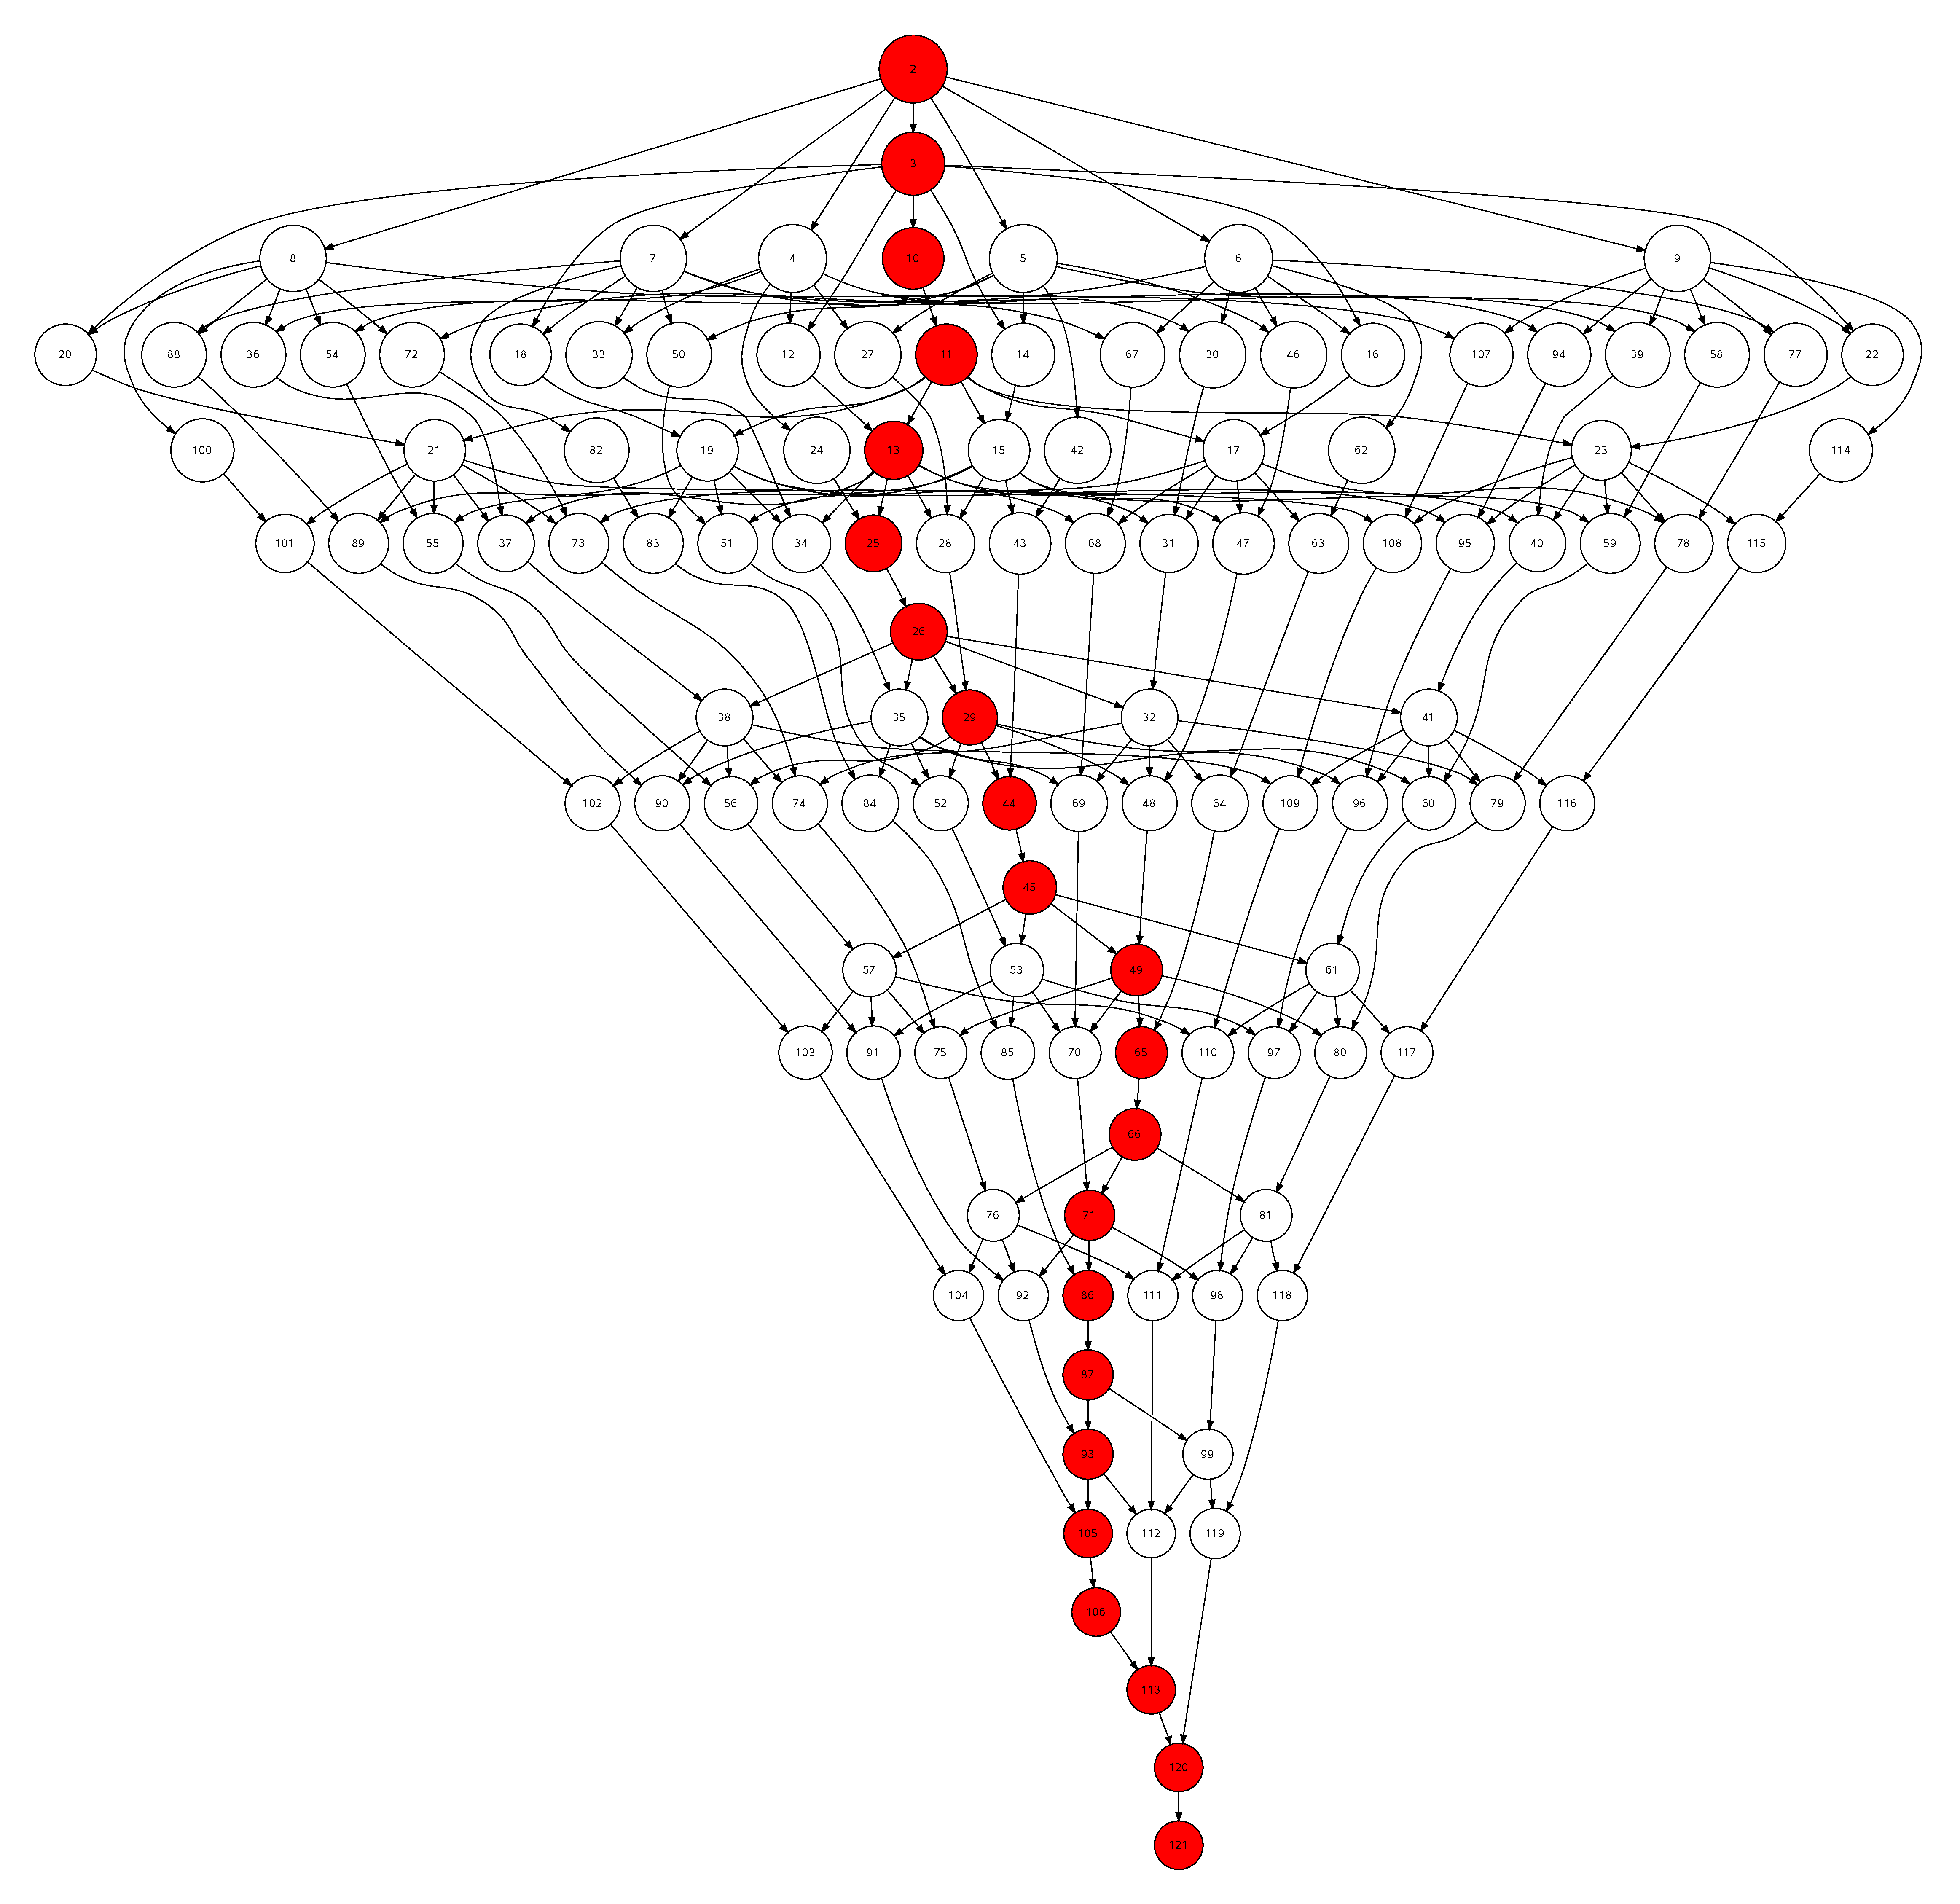
\includegraphics[width=0.26\textwidth]{images/cholesky_8_white.pdf}
		\label{cholesky8x8_TDG}
	}
	\subfloat[Cholesky 16$\times$16]{
		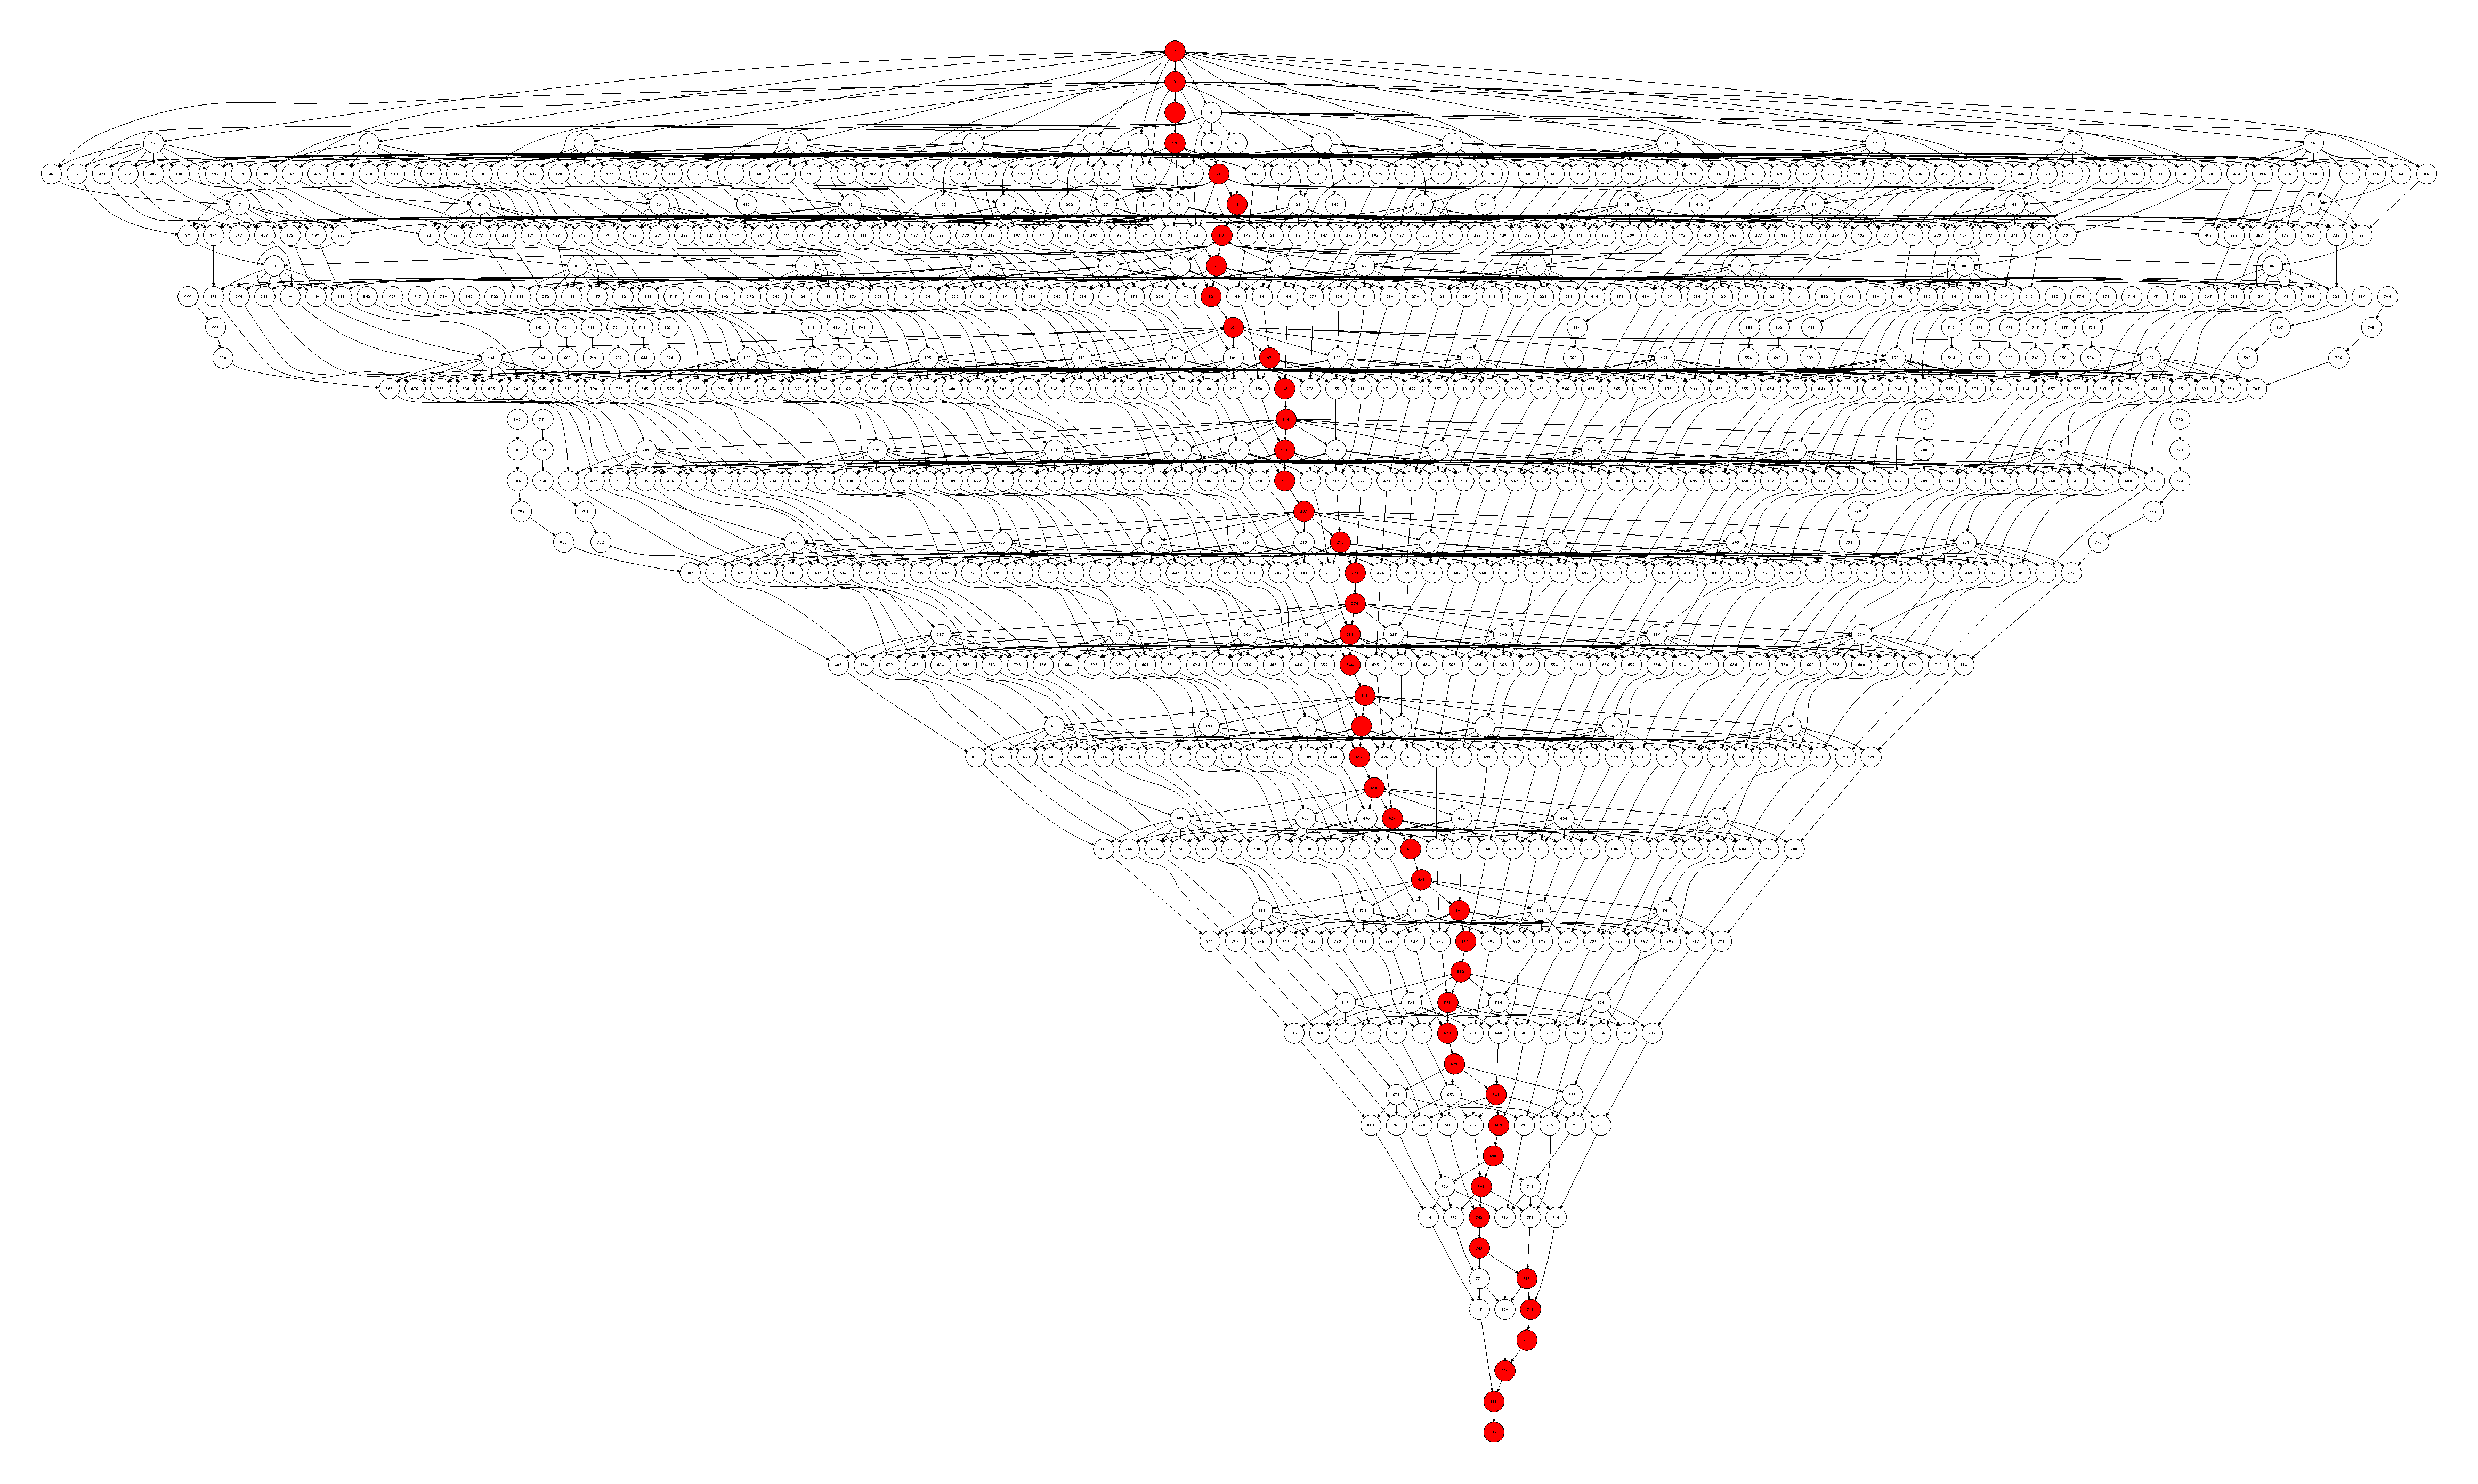
\includegraphics[width=0.6\textwidth]{images/cholesky_16_white.pdf}	
		\label{cholesky16x16_TDG}
	}
	\caption{Cholesky factorization task dependency graphs.}
	\label{fig.cholesky_graphs}
\end{figure}
% For example, a multi-core chip with some in-order cores and some out-of-order cores. The evaluation part of this paper contains real machine evaluation as well as evaluation through simulation.

%CATS targets heterogeneous multi-core systems with cores that expose different characteristics in terms of performance and power. We perform experiments on ODROID XU3 8-core platform. The ODROID XU3, features the ARM big.LITTLE technology offering heterogeneous multi-processing. Moreover, we simulate the behaviour of our design to estimate the impact of CATS on heterogeneous systems with a larger amount of cores and different performance ratios.
%On the simulated platform we are able to set up different performance ratios between fast and slow cores without a restriction.

In the first part of our real environment evaluation, we measure the execution time of four criticality-sensitive applications using CATS ad the default OmpSs scheduler. 
We evaluate four different CATS configurations based on the options explained in Section~\ref{sec.scheduling.cats} and provide a detailed comparison between them. 
The options consist of whether the task submission policy is strict or flexible, and the type of the work stealing mechanism. 
This results in the following configurations:
\begin{itemize}
	\itemsep0em
	\item Flexible with simple work stealing (SS FLEX)
	\item Flexible with bidirectional work stealing (2DS FLEX)
	\item Strict with simple work stealing (SS STRICT)
	\item Strict with bidirectional work stealing (2DS STRICT)
\end{itemize}

\kc{should it stay or should it go???:}
The default OmpSs scheduler employs a \textit{breadth-first} policy~(BF)~\cite{Duran_schedulers_08}. The BF scheduler implements a single first-in-first-out ready queue shared among all threads. 
When a task is ready, it is inserted in the tail of the ready queue and when a core becomes available, it retrieves a task from the head of the queue. Tasks are ordered according to their ready time: the earliest ready task resides at the head of the queue. Since the ready queue is shared, there is no need for work stealing and the load is balanced automatically. BF does not differentiate among core types and assigns tasks in a first-come-first-served basis.

After the analysis of the CATS configurations we measure the execution time of five applications using CATS, CPATH, HYBRID, dHEFT and the default OmpSs BF scheduler that is explained in Section~\ref{sec.background.taskbased.ompss}. 
The execution time corresponds to the average of 10 executions of the application on each machine set-up.

%%%%%%%%%%%%%%%%%%%%%%%%%%%%%%%%%%%
\if 0 % about strict/flexible
As it is already shown in previous works~\cite{Chronaki:ICS2015}, the most efficient CATS configuration is when using the simple work stealing and flexible policy (SSFLEX).
The same applies for CPATH and HYBRID schedulers, thus the results presented in this section refer to this configuration of the schedulers. 
\fi %%%%%%%%%%%%%%%%%%%%%%%%%%%%%%%%
Our test bed comprises a real big.LITTLE processor and a simulated heterogeneous system.

%The default OmpSs scheduler employs a \textit{breadth-first} policy~(BF)~\cite{Duran_schedulers_08}. The BF scheduler implements a single first-in-first-out ready queue shared among all threads. When a task is ready, it is inserted in the tail of the ready queue and when a core becomes available, it retrieves a task from the head of the queue. Tasks are ordered according to their ready time: the earliest ready task resides at the head of the queue. Since the ready queue is shared, there is no need for work stealing and the load is balanced automatically. BF does not differentiate among core types and assigns tasks in a first-come-first-served basis. We use this scheduler as a baseline for the evaluation.

%%TODO this needs to be rephrased and more structured...
%We implement a dynamic version of HEFT scheduler (dHEFT) in the OmpSs programming model. The implementation assumes two different types of cores (big and little) and keeps records of the tasks' execution times in each core. The original HEFT \cite{HEFT} implementation assumes the prior knowledge of the TDG as well as the costs of the tasks. In our case, since the evaluation consists of running benchmarks, best way to compare HEFT and the other approaches is to keep the scheduling idea of HEFT and transform it from a static scheduler to a dynamic scheduler. This means that during runtime dHEFT discovers the costs of the tasks, computes a mean value of the costs for each task-type, parameter-size duple for each type of processor and then finds the processor that will finish the task at the earliest possible time. A difference between the static HEFT and dHEFT is the order that the tasks are being submitted. In HEFT tasks are submitted in decreasing order of their upward rank, which is computed statically with the known task costs. Since dHEFT discovers the costs while tasks are executing, there is no priority in the task submission. In dHEFT tasks are submitted as soon as they become ready. To find the earliest possible executor, dHEFT maintains one list per core (\textit{wlist}) with the ready tasks that are waiting to be executed by this core. When a task is submitted, dHEFT first checks if there are records of prior execution of this task. If the number of records is sufficient (in our experiments we use 3 records at least) then the estimated execution time of the task is considered stable. So, the task is scheduled to the earliest executor by consulting the \textit{wlist} of all the processors. If the number of records is not sufficient for one of the processor types then the task is scheduled to the earliest executor of this processor type. In any case dHEFT creates history by storing every time the task cost in the appropriate records in order to maintain stable results in the next submissions.

To perform our experiments, we use the Hardkernel \textbf{Odroid-XU3} development board that has an 8-core Samsung Exynos 5422 with an ARM big.LITTLE architecture. 
This platform is described in detail in section~\ref{sec.background.arm}.
%The Hardkernel \textbf{Odroid-XU3} development board has an 8-core Samsung Exynos 5422 chip with an ARM big.LITTLE architecture and 2GB of LPDDR3 RAM at 933MHz. The chip has four Cortex-A15 cores clocked at 1.6GHz and four Cortex-A7 cores at 800MHz. The four Cortex-A15 cores form a \textit{cluster} with a shared 2MB L2 cache, and the Cortex-A7 share a 512KB L2 cache. The two \textit{clusters} are coherent, so a single shared memory application can run on both clusters, using up to eight cores simultaneously. 
In our experiments, we evaluate a set of possible combinations of fast and slow cores varying the total number of cores from two to eight. 
%For the remainder of this section, we refer to Cortex-A15 cores as \textit{big} and to Cortex-A7 cores as \textit{little}.

% Talking about the performance ratio of the applications before describing the applications sound a bit strange, let's move this to applications section
%Depending on the workload, big and little cores expose different performance ratios. For example, a double precision benchmark advances a big core to be 3$\times$ faster than a little core, while for integer operations a big core is 1.9$\times$ faster than a little one \cite{Greenhalgh2011}. To get the notion of this performance ratio, we perform an execution of each application in one big core and another identical execution in one little core. The difference in performance on these two execution defines the difference in performance for big and little cores for each specific workload. Table \ref{tab.apps} shows the performance ratios explored for the benchmarks that we use.

%According to the calculated performance ratio, we can export the upper bound on speedup over a little core for each benchmark when running on 8 cores. Equation \ref{eq.ideal} shows how the ideal speedup is computed and assumes that the workload can be fully parallelized with zero dependencies, overheads or sequential sections in the application, according to Amdahl's law \cite{Amdahl}.
%\begingroup\makeatletter\def\f@size{9}\check@mathfonts
%\begin{equation}
%  \text{IDspeedup(workload, 8) = 4 $\times$ perf\_ratio(workload) + 4}
%\label{eq.ideal}
%\end{equation}
%\endgroup


%% Replaced for anonimity
%\subsubsection{TaskSim}

%Heterogeneous platforms such as ODROID-XU3 are currently limited in terms of size. We expect that future heterogeneous platforms will grow bigger with a larger amount of cores and various performance differences between fast and slow cores. 
To evaluate heterogeneous scheduling on larger multi-core systems we use the heterogeneous multi-core TaskSim simulator~\cite{AbstrLevels_TACO12} described in section~\ref{sec.background.simulation}. TaskSim allows the specification of a heterogeneous system with two different types of cores: fast and slow. 
We can configure the amount of cores of each type and the difference in performance between the different types (performance ratio) in the TaskSim configuration file.
In our experiments, we evaluate the effectiveness of the schedulers on 8 distinct heterogeneous machine configurations. 
These comprise systems with 16 or 32 total number of cores, and the number of fast cores ranging from 1 to 16. 
We set the performance ratio between fast and slow cores to 4.5$\times$ because this is the average performance ratio observed on the real machine for the benchmarks of this evaluation.

%For all these configurations, we evaluate the following performance ratios between fast and slow cores: 2$\times$, 2.5$\times$, 3$\times$, 3.5$\times$ and 4$\times$.

%% moved here because we needed to know about the heterogeneous platforms before talking about big and little cores

%The metric used in the following charts for each pair (\textit{total number of cores, number of big cores}), is the improvement of CATS over the baseline scheduler as well as the speedup obtained for each policy over one LITTLE core. The improvement is computed as shown in Equation~\ref{eq.improvement} and the speedup is computed as shown in Equation~\ref{eq.speedup}.

%% This, we are already saying in the explanation of the platforms
%

For both real and simulated platforms, each set-up has a given number of \textit{total} and \textit{big} cores.
%Our metrics are the improvement of CATS over the baseline scheduler, and the 
For all the scheduling approaches we present their speedup over the execution on one \textit{little} core, shown in Equation~\ref{eq.sched.speedup}. 
%Equations~\ref{eq.improvement} and~\ref{eq.speedup} show the improvement and speedup calculations.
%Equation~\ref{eq.speedup} shows how speedup is calculated in this evaluation.
\begingroup\makeatletter\def\f@size{8}\check@mathfonts
%\begin{equation}
%  \text{Improv. over BF(total, big)} = \frac{\text{Exec. time BF(total, big)}}%{\text{Exec. time CATS(total, big)}}
%\label{eq.improvement}
%\end{equation}
\begin{equation}
  \text{Speedup(total, big)} = \frac{\text{Exec. time(1, 0)}}{\text{Exec. time(total, big)}}
  \label{eq.sched.speedup}
\end{equation}
\endgroup


\subsubsection{Applications}

\begin{table*}
	\scriptsize
	\begin{center}
		\caption{Evaluated benchmarks and relevant characteristics. The inputs of QR and Heat diffusion are arrays of doubles and the inputs of Cholesky and Int. Histogram are arrays of floats.}
		\label{tab.sched.apps}
		\begin{tabular}{|c|c|c|c|c|c|c|c|c|}
			\hline
			\multirow{2}{*}{\parbox{10mm}{\centering Application}} & 
			\multirow{2}{*}{\parbox{9mm}{\centering Problem size}} & 
			\multirow{2}{*}{\parbox{9mm}{\centering \#Tasks}} & 
			\multirow{2}{*}{\parbox{9mm}{\centering \#Task types}} & 
			\multirow{2}{*}{\parbox{18mm}{\centering Avg task exec. time (${\mu}s$)}} & 
			\multicolumn{3}{|c|}{Per task overheads (${\mu}s$)} &\\
			\cline{6-8}
			& & & & & {\parbox{10mm}{\centering CATS}} & {\parbox{10mm}{\centering CPATH}} & {\parbox{11mm}{\centering HYBRID}} &
			
			\multirow{2}{*}{\parbox{13mm}{\centering Measured perf. ratio}} \\
			& & & & & & & & \\ %\hhline{~~~~~~}
			\hline
			
			\multirow{3}{*}{Cholesky} 
			& 8K 1024 & 120 & & 10\,314\,660 & 81.19 &  115.29 &  112.41 & \\                                              
			& 8K 512 & 816 & 4 & 1\,551\,322 & 104.76 &  238.02 &  194.28 &3.48 \\ 
			& 16K 512 & 5984 & & 1\,551\,322 & 104.76 &  238.02 &  194.28  & \\ 
			\hline{}
			QR & 8K 512 & 1\,496 & 4 & 11\,651\,079  &   1\,419.33 & 2\,580.41 &   1\,451.74 & 6.86 \\ 
			\hline
			Heat diffusion & 8K 512 & 5\,124 & 3 & 93\,198  &   145.17  &  748.84 &  170.00& 3.68 \\
			\hline
			Int. Histogram & 8K 512 & 2\,048 & 2 & 514\,096 &  217.45 &  62.07 & 263.62  & 2.23 \\ 
			%Heat diffusion & Heat &  &  &  &  &  & \\ 
			\hline
			Bodytrack & native & 408\,525 &  6 & 41\,869 & 93.90 & 120.93 &  120.93 & 4.14 \\
			\hline
		\end{tabular} 
	\end{center}
\end{table*}
\normalsize
\begin{figure}[t]
	\centering
	\subfloat[Cholesky 8$\times$8]{
		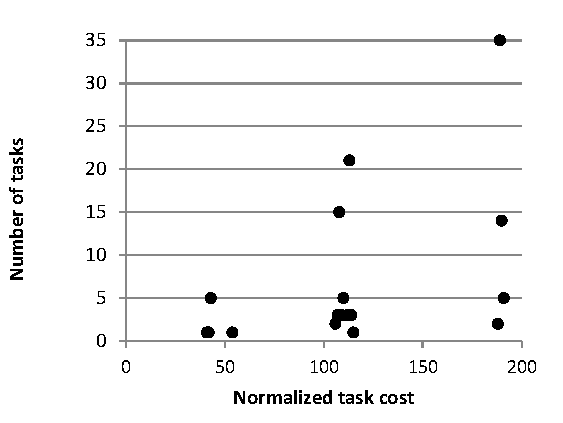
\includegraphics[width=0.3\textwidth]{images/cholesky_8x8_distribution.pdf}
		\label{cholesky8x8_dist}
	}
	\subfloat[Cholesky 16$\times$16]{
		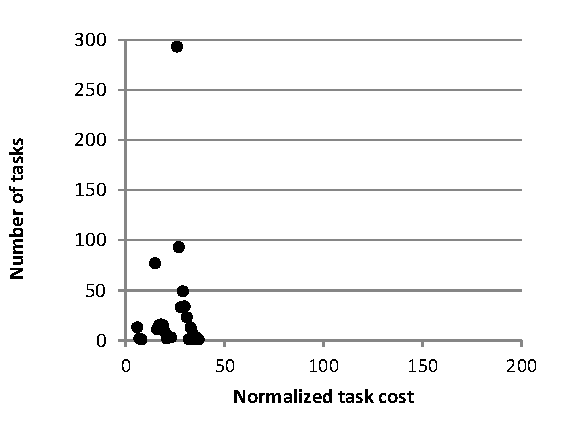
\includegraphics[width=0.3\textwidth]{images/cholesky_16x16_distribution.pdf}	
		\label{cholesky16x16_dist}
	}
	\subfloat[QR factorization]{
		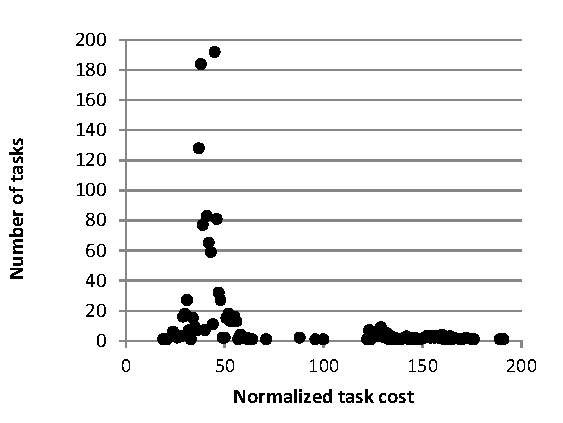
\includegraphics[width=0.3\textwidth]{images/QR_16x16_distribution.pdf}	
		\label{qr_dist}
	}
	\\
	\subfloat[Heat diffusion]{
		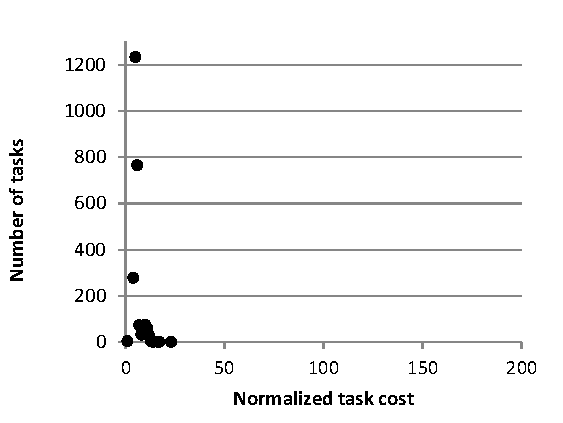
\includegraphics[width=0.3\textwidth]{images/heat_16x16_distribution.pdf}	
		\label{heat_dist}
	}
	\subfloat[Integral Histogram]{
		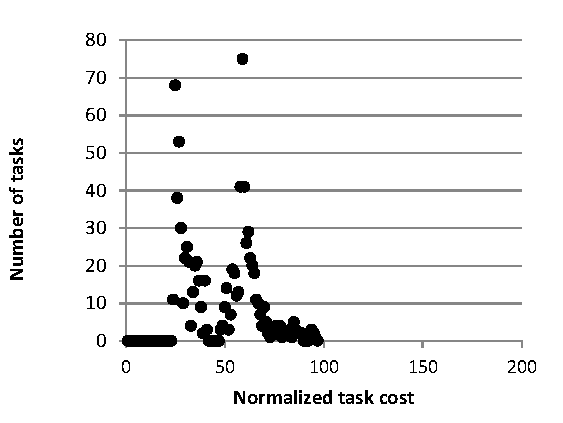
\includegraphics[width=0.3\textwidth]{images/histogram_8x8_distribution.pdf}	
		\label{histogram_dist}
	}
	\subfloat[Bodytrack]{
		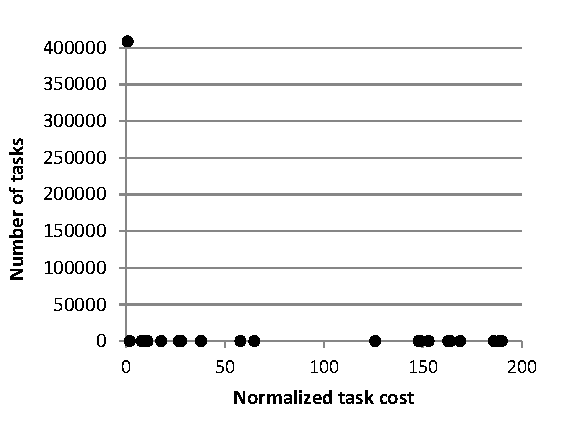
\includegraphics[width=0.3\textwidth]{images/bodytrack_native_distribution.pdf}	
		\label{bodytrack_dist}
	}
    \caption{Task cost distribution for each application. Results are based on 4BIG-core executions. $x$ axis shows the cost of the tasks and $y$ axis shows the number of tasks with the corresponding task cost.}
  \label{distributions}
  %\vspace{-0.4cm}
\end{figure}

We use five scientific applications implemented in the OmpSs programming model: Cholesky factorization, QR factorization, Heat diffusion, Integral Histogram and Bodytrack, also described in Section~\ref{sec.background}. 
These benchmarks are accessible in the BSC Application Repository~\cite{BAR} and in the PARSECSs library~\cite{Chasapis:TACO2016}. 


%\subsubsection{Bodytrack}
%\textbf{Bodytrack} is an application that tracks a marker-less human body using multiple cameras through an image sequence. 
%The OmpSs version implements a two-stage parallel pipeline for the image processing.
%%In the first stage the implementation allows the concurrent processing of all the frames of the image sequence. 
%%The second stage is the application of a particle filter to the images in order to mark the human body.
%The two stages are synchronized through the OmpSs dataflow annotations.
%By allowing the parallel processing of frames, OmpSs achieves the overlapping of the I/O and serial code with the tasks. 
%We use the native input of the benchmark suite~\cite{Chasapis:TACO2016}.

%Their different configurations and characteristics are shown in Table~\ref{tab.apps}.
%
%The applications have different sensitiveness depending on the inter-task dependencies that determine the available parallelism and the percentage of critical tasks, shown in the table. The larger proportion of critical tasks, the larger the potential improvement of CATS, as these are tasks that, once accelerated, reduce the application overall execution time. The percentage of critical tasks in Table~\ref{tab.apps} is from a single-core execution of CATS. Since CATS is dynamic, the tasks considered critical would be different for different configurations, since the algorithm runs on a partial dependency graph, including only the outstanding tasks. However, the single-core figures serve as an estimation of the percentage of critical tasks intrinsic to the overall application, that allows us to reason about the results with respect to this application characteristic.
%
%The percentage of critical tasks characterises the shape of the task dependency graph. The larger the proportion of critical tasks, the narrower the graph. These percentages, are exported from a single-core CATS execution of each kernel. So, this shows the theoretical amount of critical tasks that CATS discovers, since a multi-core execution of the application would detect the longest path dynamically. Nevertheless, it is shown experimentally that an application with a higher theoretical percentage of critical tasks has a higher number of critical tasks in practice, than an application with a small theoretical percentage of critical tasks.
%
%Depending on the workload, big and little cores expose different performance ratios. For example, a double precision benchmark advances a big core to be 3$\times$ faster than a little core, while for integer operations a big core is 1.9$\times$ faster than a little one \cite{Greenhalgh2011}. To get the notion of this performance ratio, we perform an execution of each application in one big core and another identical execution in one little core. The difference in performance on these two execution defines the difference in performance for big and little cores for each specific workload. Table \ref{tab.apps} shows the performance ratios explored for the benchmarks that we use.
%IDEAL SPEEDUP
%The performance ratios in Table~\ref{tab.apps} are computed for the real machine by comparing the execution time on one little core over the execution time on one big core. Using these performance ratios, we can estimate the ideal speedup over a little core for each application running on all eight cores. Equation~\ref{eq.ideal} is used for the ideal speedup. The ideal speedup considers a fully parallel workload, without any dependencies, overheads or sequential sections, thus unachievable by the dependency-intensive applications in our evaluation.%in the application, according to Amdahl's law \cite{Amdahl}.
%\begingroup\makeatletter\def\f@size{7}\check@mathfonts
%\begin{equation}
%  \text{ideal\_speedup(workload, 8) = 4 $\times$ perf\_ratio(workload) + 4}
%\label{eq.ideal}
%\end{equation}
%\endgroup
%END IDEAL SPEEDUP

Table \ref{tab.sched.apps} shows the different configurations and characteristics of the applications.
For cholesky, QR, heat diffusion and integral histogram the input is a square matrix divided into blocks.
The \textit{Problem size} column of Table~\ref{tab.sched.apps} shows the dimension of the input matrix and the block size.
For example cholesky 8K 1024 takes as input a matrix of 8192$\times$8192 and it is then divided to 8$\times$8 blocks of 1024 elements each.
Each task created in the parallelized versions operates on one block.
The bigger the block size, the less the number of blocks created, which leads to less tasks. 
From the applications of Table~\ref{tab.sched.apps}, QR and Heat diffusion operate on doubles while Cholesky and Integral Histogram operate on floats.
The performance ratio between big and little cores depends on the application. 
For example, the difference between the issue rate and throughput of double-precision floating point units of both types of cores is larger than the difference for single-precision floating point instructions. Therefore, applications with heavy double-precision operation (e.g. QR) get a larger benefit from running on the big cores, than single-precision dominated applications (e.g integral histogram), as shown in Table~\ref{tab.sched.apps}.

The average per task overhead for each scheduler is negligible compared to the average task execution time shown in Table~\ref{tab.sched.apps}. Specifically, CATS has the lowest per task overheads. Next is HYBRID and the least efficient is CPATH. This is because of the complexity of the CPATH algorithm that takes place whenever the TDG needs to be updated.
On the other hand, CATS and HYBRID have negligible overheads caused by the task prioritization.
For dHEFT, the search of the appropriate worker for a task becomes an obstacle in performance. 
Table~\ref{tab.sched.apps} lacks the per task overheads of dHEFT because they appear to be too high due to the fact that the most intensive computations of dHEFT take place during the cores' idle time.
Thus, the natural idle time of cores is also encountered as scheduling overhead and could not be separated, so it is unfair to present such results for comparison. 
Normally these obstacles in heterogeneous schedulers are paid off by the more effective task execution. 

Figure~\ref{fig.cholesky_graphs} shows the TDGs for input sizes of (a) 8$\times$8 and (b) 16$\times$16 blocks.
Critical tasks are denoted as red nodes. 
The TDG becomes wider as the number of blocks increases. 
This reduces the percentage of critical tasks that is 17.5\% in the case of the 8$\times$8 input and 5.51\% in the case of the 16$\times$16 input. 
The 8$\times$8 blocks case shows a narrower TDG that makes the application more criticality sensitive than the 16$\times$16 blocks case that exposes more parallelism. 
We evaluate both configurations to show the impact of scheduling on different criticality sensitiveness of the application configuration.

To more precisely characterise the benchmarks, we plot the task cost variability for each benchmark on Figure~\ref{distributions}.
We normalize the task execution time of the applications with respect to the smaller task observed among all applications so that we can easily compare the task sizes of different applications as shown on the distributions.
For each of these plots, the $x$ axis shows the normalized task cost (i.e. task execution time) and the $y$ axis the number of tasks that correspond to this task cost (e.g. how many tasks have this cost).
This is used in the next section to classify how heterogeneous each application is and explain the behavior of the heterogeneous schedulers that take into account the execution time.
%\subsubsection{Cholesky Factorization}



%\begin{figure*}[!t]
%	\centering
%	
%		\begin{subfigure}[b]{0.45\textwidth}
%		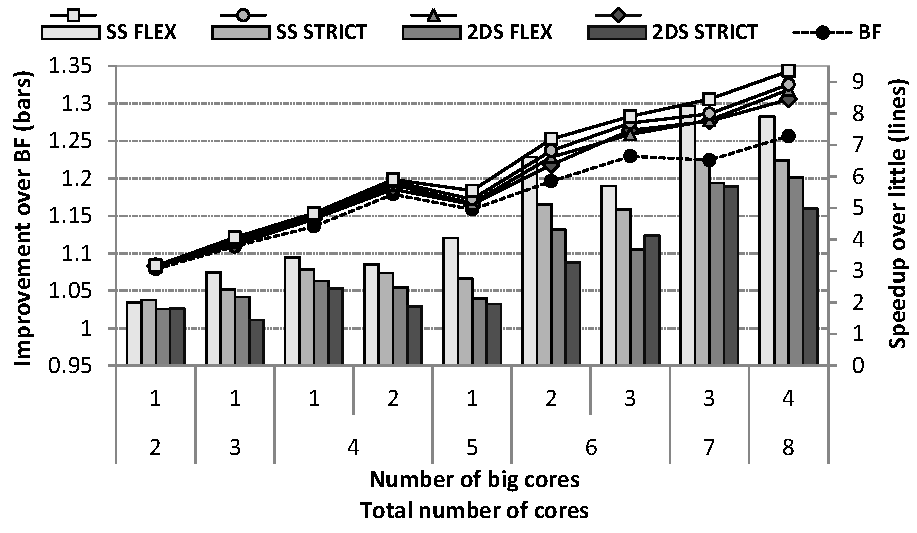
\includegraphics[width=\textwidth]{figures/cholesky_8x8_CATS.pdf}
%		\caption{Cholesky 8$\times$8}
%		\label{cholesky8x8_real}
%	\end{subfigure}
%	\begin{subfigure}[b]{0.45\textwidth}
%		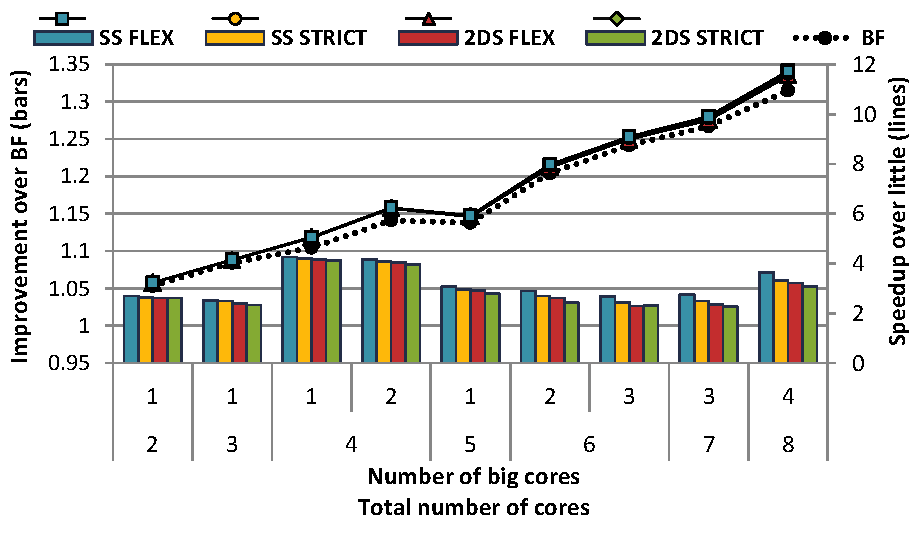
\includegraphics[width=\textwidth]{figures/cholesky_16x16_CATS.pdf}
%		\caption{Cholesky 16$\times$16}
%		\label{cholesky16x16_real}
%	\end{subfigure}
%	\begin{subfigure}[b]{0.45\textwidth}
%		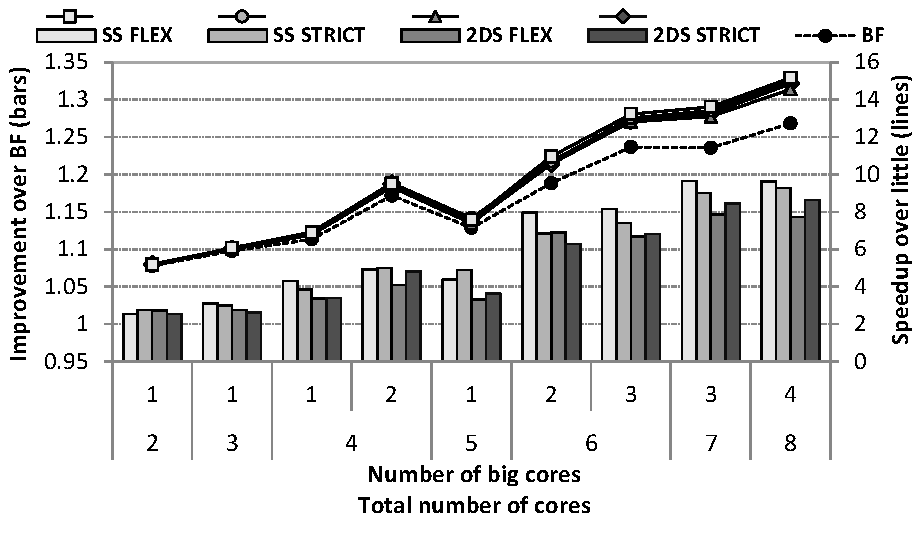
\includegraphics[width=\textwidth]{figures/QR_CATS.pdf}
%		\caption{QR}
%		\label{qr_real}
%	\end{subfigure}
%	\begin{subfigure}[b]{0.45\textwidth}
%		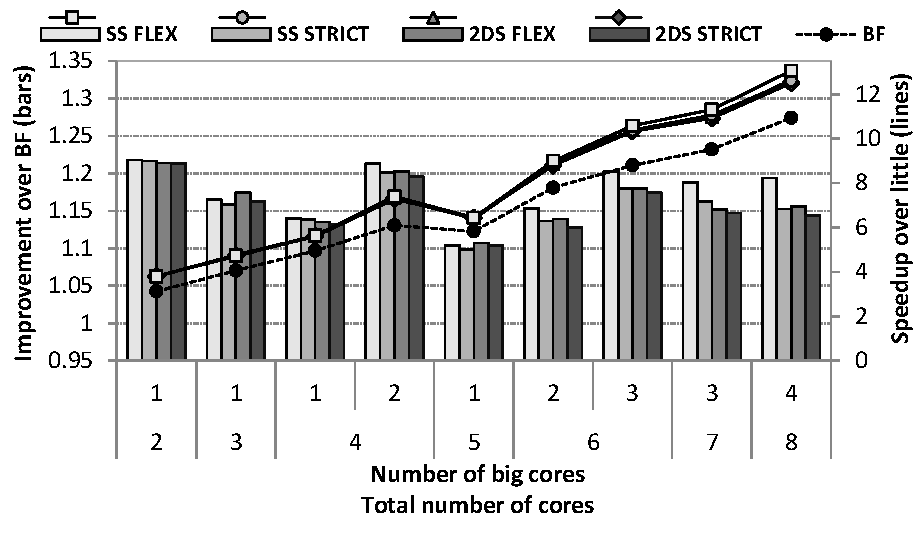
\includegraphics[width=\textwidth]{figures/heat_CATS.pdf}
%		\caption{Heat Diffusion}
%		\label{heat_ARM}
%	\end{subfigure}
%	\begin{subfigure}[b]{0.45\textwidth}
%		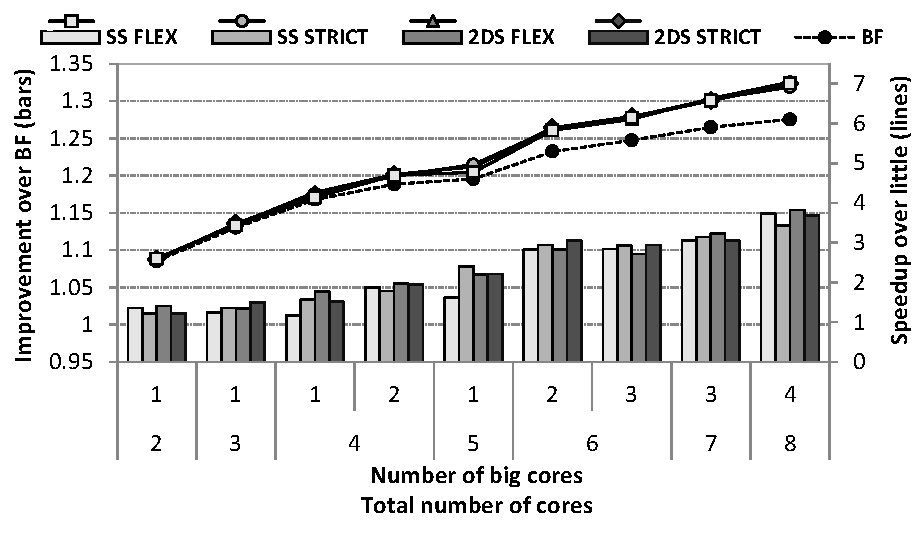
\includegraphics[width=\textwidth]{figures/intHist_CATS.pdf}
%		\caption{Integral Histogram}
%		\label{histogram_real16}
%	\end{subfigure}
%	\caption{Schedulers comparison on ODROID-XU3}
%	\label{eval_ARM}
%	\vspace{-0.4cm}
%\end{figure*}

\subsection{Real Environment Evaluation}
This subsection includes all the experiments and results obtained from the real asymmetric system ODROID-XU3.
It includes one section that explores the different CATS configurations and another section that compares the best CATS configuration among the rest of the schedulers.

\subsubsection{Evaluation of CATS Configurations}
\label{sec.cats_eval}
\begin{figure}[!t]
	\centering
		\subfloat[Speedup of CATS and BF compared to the ideal]{
		\includegraphics[width=0.45\textwidth]{figures/ideal_CATS.pdf}
		\label{BFlinear}
	}
	\subfloat[Cholesky 8$\times$8]{
		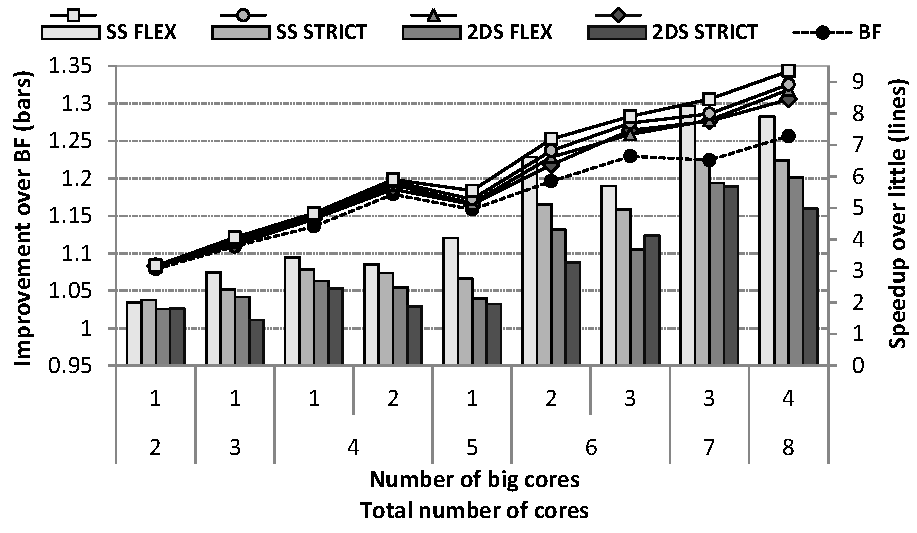
\includegraphics[width=0.45\textwidth]{figures/cholesky_8x8_CATS.pdf}
		\label{cholesky8x8_cats}
	}
	\\
	\subfloat[Cholesky 16$\times$16]{
		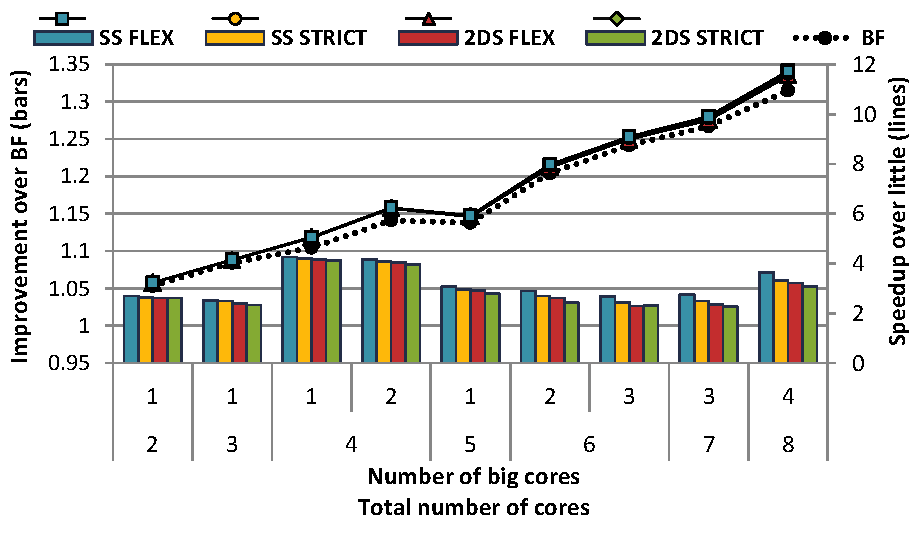
\includegraphics[width=0.45\textwidth]{figures/cholesky_16x16_CATS.pdf}
		\label{cholesky16x16_cats}
	}
	\subfloat[QR]{
		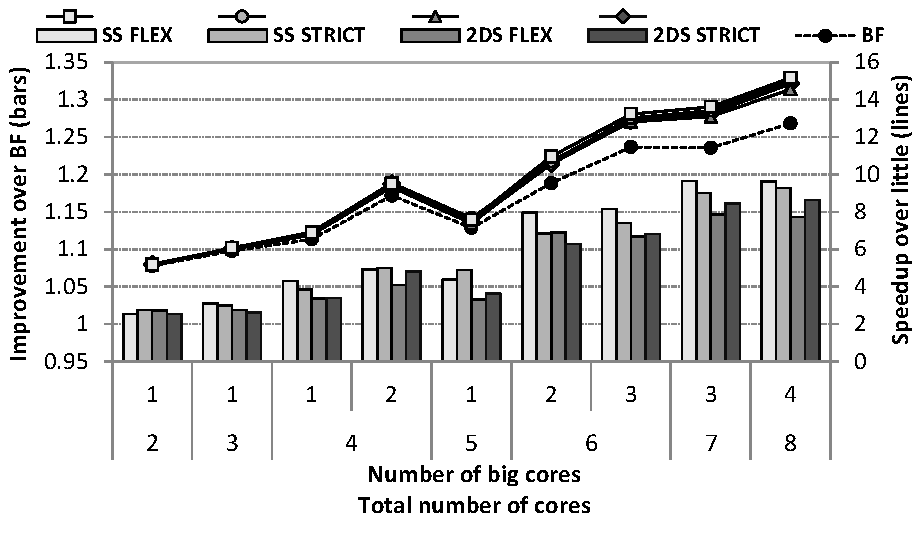
\includegraphics[width=0.45\textwidth]{figures/QR_CATS.pdf}
		\label{qr_cats}
	}
	\\
	\subfloat[Heat diffusion]{
		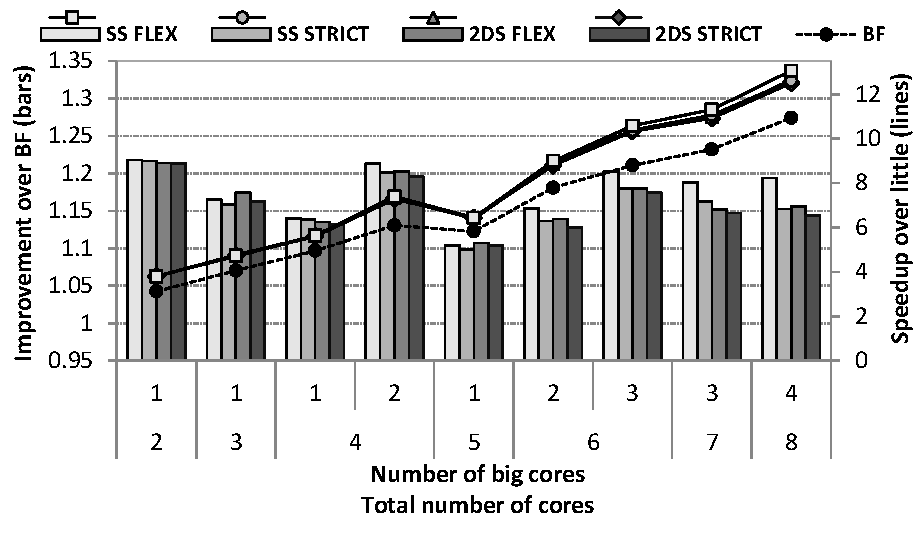
\includegraphics[width=0.45\textwidth]{figures/heat_CATS.pdf}
		\label{heat_cats}
	}
	\subfloat[Integral Histogram]{
		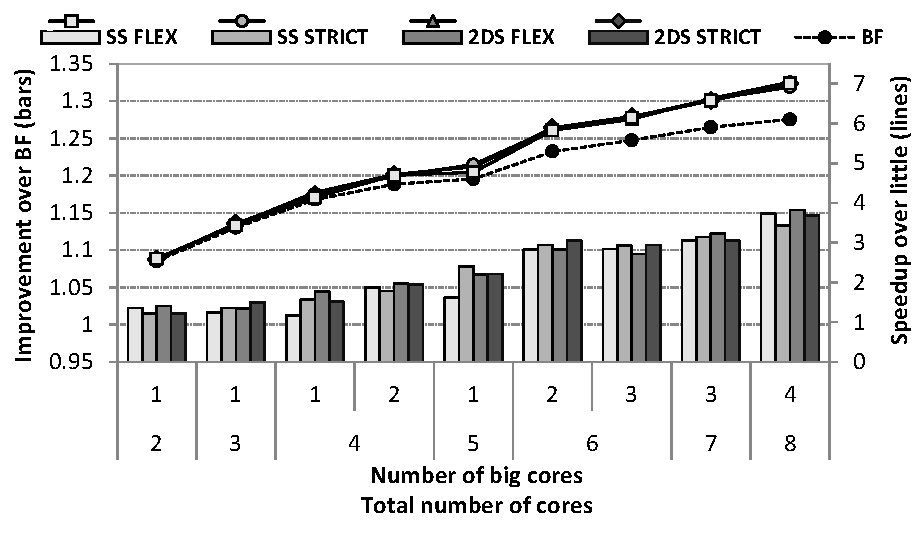
\includegraphics[width=0.45\textwidth]{figures/intHist_CATS.pdf}
		\label{histogram_cats}
	}
	%  \vspace{-0.2cm}
	\caption{Schedulers comparison on ODROID-XU3}
	%\vspace{-0.5cm}
\end{figure}
Figure~\ref{cholesky8x8_cats} shows the improvement of the CATS configurations over BF, and the speedup obtained with CATS and BF, for Cholesky on an 8$\times$8 blocked matrix. 
CATS consistently achieves better performance than BF and the improvement over BF increases as the number of cores is increased. 
Specifically, the improvement is observed to be up to 30\% for systems with seven and eight cores. 

Figure~\ref{cholesky16x16_cats} shows the performance on a 16$\times$16 block input matrix, where the improvement of CATS is smaller and ranges from 2 to 9\% and all schedulers perform fairly well. 
In this case the opportunities for enhancement are limited, since, according to Figure~\ref{BFLinear}, BF performance approaches the ideal speedup. 
The lower improvement in this case comes from the fact that the application is less sensitive to the critical path. 
The task graph is wider (as shown in Figure~\ref{fig.cholesky_graphs}) and, accordingly, the percentage of critical tasks is lower. 
Specifically the percentage of critical tasks for this input is limited to 5.5\% compared to the percentage observed with Cholesky 8$\times$8 that is 17.5\%. 
However, CATS still outperforms BF by 7\% when using the eight cores in the system.% and performs as good as dHEFT.

%It is interesting to note that the proportion of critical tasks, as shown in Table~\ref{tab.apps}, is lower than in the previous experiment, which leads to a lower utilization of the big cores for critical task execution.

Figure~\ref{qr_cats} shows the improvement of CATS over BF and their speedup for QR factorization. 
QR consists of double precision operations which cause the big cores to be 4.26$\times$ faster than the little cores. Thus, the ideal speedup of the system for QR is 20.1$\times$. 
CATS achieves a 15$\times$ speedup by shortening the execution of the dynamic longest path in the TDG. 
%Since dHEFT is not focusing on the longest path of the TDG, and it performs some random scheduling at the beginning of the execution in order to determine the task costs, it becomes less effective than CATS but still better than a BF.

Figure~\ref{heat_cats} shows the improvement of different CATS configurations over BF, and the speedup obtained with CATS and BF, for heat diffusion. 
%As shown in Table~\ref{tab.apps} heat diffusion consists of 5124 tasks; 5120 tasks of them are tasks of the same type and parameter size. 
%This limits the effect of dHEFT, that tries to find the earliest executor for each task in comparison to BF in which whenever a core becomes available, it retrieves a task from the ready queue. Thus, dHEFT is better than BF because it uses private ready queues for each core, thing that reduces the congestion of using only one ready queue. 
CATS consistently improves the scheduling of the asymmetric system from 15\% to 22\%, since the main criterion of scheduling is the TDG structure. 
CATS achieves a 13$\times$ speedup when using all eight cores, thus getting very close to the ideal 15.3$\times$ shown in Figure~\ref{BFLinear}.

Figure~\ref{histogram_cats} shows the improvement of CATS over BF, and the speedup obtained with CATS and BF, for integral histogram. 
The impact of CATS is again positive for all configurations, since the improvement is at least 5\% with the peak being 15\% for 8 cores. 
Experiments on larger systems show that the specific application's scalability saturates beyond 16 cores. 
This is because the intensive dependencies between tasks reduce the available parallelism that is mainly present among the diagonal-placed blocks due to the cross-weave scanning process. 
%Since dHEFT does not take into account the dependencies between tasks, the scheduling of an application with limited parallelism due to dependencies becomestrickier. 
Moreover, the performance ratio of this single-precision application is 1.7$\times$, so the ideal speedup is limited to 10.8$\times$.

An interesting observation is that for single-precision benchmarks the improvement of CATS is proportional to the percentage of critical tasks. 
Integral histogram achieves greater improvements in comparison to Cholesky 16$\times$16 because it schedules immediately more tasks to the fast cores of the system.
This is due to the fact that this benchmark has a higher percentage of critical tasks (7.32\%) compared to Cholesky 16$\times$16 that has 5.5\%. 
%according to the percentage of the critical tasks on Table \ref{tab.apps}. 
On the other hand, QR and heat diffusion show the opposite effect: QR has the largest performance ratio and a larger percentage of critical tasks than heat diffusion. 
However, heat diffusion shows higher overall improvement over the different configurations. 
We attribute this to the larger sensitivity of heat diffusion to the critical path, which allows CATS to achieve a large improvement even for a configuration of one big and one little core. 
%The dHEFT scheduler outperforms BF but struggles to handle applications with complex TDG. 
%Applications that consist of multiple instances of the same task type benefit less from dHEFT than applications that process tasks with variable costs, such as Cholesky and QR. 

In all cases, the SS FLEX configuration of CATS achieves the best performance, since it produces a decent amount of critical tasks for the big cores, fact that shortens the longest path of the TDG. 
A smaller amount of critical tasks is produced by the SS STRICT policy, which causes a slight imbalance that is fixed through the work stealing mechanism but with lower effectiveness. 
The 2DS FLEX configuration, produces the same amount of critical tasks as the SS FLEX, but the bi-directional work stealing allows little cores to steal critical tasks, which lengthens the critical path execution and directly increases overall execution time.

\subsubsection{Evaluation of CATS CPATH and HYBRID}
\begin{figure}[!t]
	\centering
	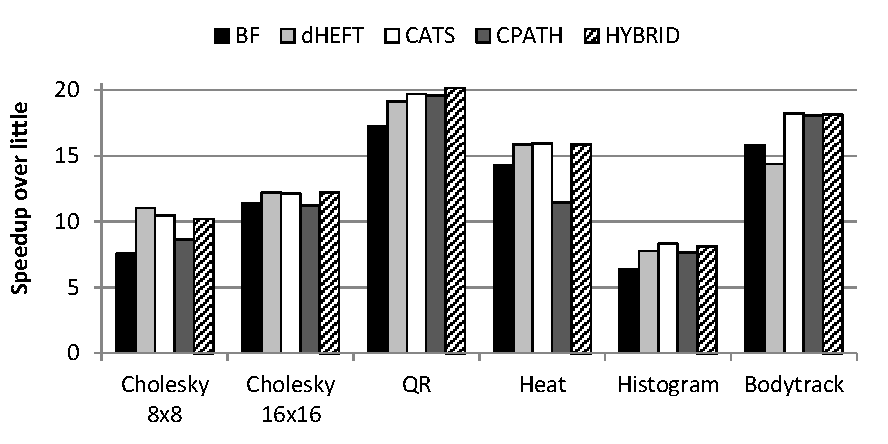
\includegraphics[width=0.7\textwidth]{images/8cores.pdf}
	\caption{Speedup of CATS, CPATH, HYBRID, dHEFT and BF on 8 cores compared to the ideal}
	\label{BFLinear}
	\vspace{-0.4cm}
\end{figure}
As it is shown in Section~\ref{sec.cats_eval}, the most efficient CATS configuration is when using the simple work stealing and flexible policy (SSFLEX).
The same applies for CPATH and HYBRID schedulers, thus the results presented in this section refer to this configuration of the schedulers. 
Figure~\ref{BFLinear} shows the speedup of CATS, CPATH, HYBRID, dHEFT and BF when running the applications on all eight cores of the Odroid-XU3. Cholesky and Integral Histogram operate on single-precision data, while QR and Heat Diffusion operate on double-precision. 
Double-precision applications get larger speedups over one little core because they benefit from a larger performance ratio when running on a big core. In the case of Bodytrack, the out-of-order processing power of the big cores helps on the efficient execution and creates a high performance ratio between big and little cores. 
For most of the cases, CATS scales better than the rest of the schedulers. 
The shortening of the critical path by running all critical tasks on big cores effectively reduces total execution time when running on all cores. 
CPATH scheduler does not achieve as high speedup as the other heterogeneous scheduling approaches but it still outperforms the baseline (BF) approach.

Figure~\ref{avg_all} shows the average speedup obtained for each scheduler and machine set-up. 
Overall, the heterogeneous schedulers outperform the platform-unaware BF scheduler.
Specifically, CATS and HYBRID achieve a higher speedup by detecting critical tasks.
We observe that their performance is approximately the same and this is due to the fact that HYBRID exploits the same CATS criticality in case the execution time of the task is not yet resolved.
CPATH is less effective due to the additional overheads of the top-to-bottom TDG traversal.
Since the evaluated dHEFT version is improved from previous studies~\cite{Chronaki:ICS2015}, it shows better performance, although it still does not reach the efficiency of CATS and HYBRID because of its task criticality agnosticism.

Moving in more detail, Figure~\ref{speedup} shows the speedup obtained for each application,  scheduler and machine set-up.
We classify the benchmarks according to their task cost variability to easier explain the results.

%------ HEAT ---------- very low variability


Heat diffusion is the kernel with the lowest task variability (e.g. the most homogeneous benchmark) as shown in Figure~\ref{heat_dist}.
CATS, HYBRID and dHEFT increase the performance of heat by 10\% on 8 cores and obtain similar results for the other numbers of cores by rearranging the tasks according to the type of the resources.
Due to its high per-task overheads shown on Table~\ref{tab.sched.apps}
%(CATS: 145.17us per task, CPATH: 748.84us per task, BF: 78.04us per task HYBRID: 170us per task)
 and the homogeneity of the benchmark, CPATH scheduler cannot outperform BF scheduler. 
Moreover, for this benchmark, CPATH detects only 23\% of the tasks to be critical while CATS and HYBRID detect approximately 54\%, when running on 8 cores.
This happens because with CPATH, it is more likely to have zero-priority tasks during the task submission step, due to the post-exit task priority assignment that the algorithm introduces. 
These tasks are considered non-critical, which limits the utilization of the big cores with CPATH. 
%the priorities of the tasks are computed more slowly with CPATH so during task submission there are many tasks with zero priority that are considered non-critical.
%Moreover, as Table~\ref{tab.critical} shows CPATH detects only 23\% of the tasks to be critical while CATS and HYBRID both detect approximately 54\% when running on 8 cores. 
%This limits the utilization of the big cores with CPATH.

%---------- CHOLESKY 16x16 ------------ low variability

Cholesky 16$\times$16 has also low task cost variability. 
The improvements of CATS, dHEFT and HYBRID over BF are limited to around 7\% when running on 8 cores.
These schedulers perform almost the same for the rest numbers of cores and CPATH performs almost the same as BF. 
The increased overheads of CPATH do not pay off with better schedules since, for the same reason as in the case of Heat diffusion, only 10\% of the tasks are marked as critical on 8 cores (while 21\% CATS and 16\% HYBRID).

%--------- BODYTRACK --------------- low variability - very high number of tasks

Bodytrack shows low task cost variability, since 99\% of its tasks have similar execution times.
In this case, contrarily to the previous benchmarks CPATH manages to achieve similar speedups to CATS and HYBRID and outperform BF by up to 15\%.
This is due to the very high number of tasks of bodytrack; CPATH overcomes its overheads by using the detected task execution times for a higher number of tasks.
In other words, the learning phase of CPATH becomes a smaller proportion of the total execution of the benchmark.
Since bodytrack has so many tasks, the per-task overhead of CPATH is around 120us while for CATS it is 93us.
On the other hand, dHEFT shows poor performance because of the overheads of analyzing a TDG with a high number of tasks to compute the earliest finish time schedule.

\begin{figure}[!tr]
	\centering
  	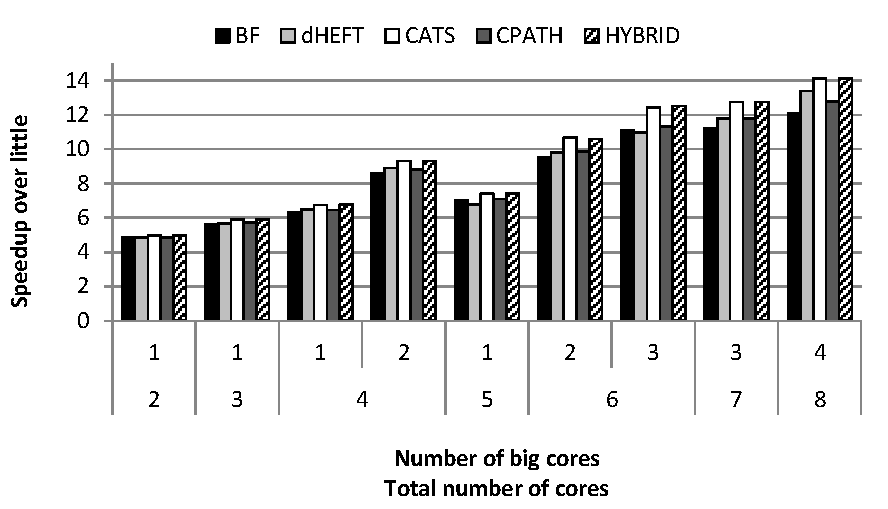
\includegraphics[width=0.7\textwidth]{images/average_all.pdf}
  	\caption{Average speedups obtained for each scheduler}
  	\label{avg_all}
  	\vspace{-0.5cm}
\end{figure}  

%---------- HISTOGRAM --------------- medium variability - good amount of tasks (2048)

Integral histogram is characterized by medium task cost variability and high amount of tasks.
This benchmark is dependency intensive with limited parallelism, which makes scheduling decisions very important.
CATS and HYBRID schedulers achieve the best results since they focus more on the TDG structure and dependencies, improving BF by 30\% and 27\% respectively.
CPATH and dHEFT are slightly less efficient and improve BF by 19 and 21\% respectively.

%---------- CHOLESKY 8x8 -------------- high variability but very few tasks

For Cholesky 8$\times$8, the heterogeneous schedulers CATS, HYBRID and dHEFT constantly improve the performance of BF and reach up to 45\% improvement on 8 cores.
It is observed here that dHEFT indeed performs better when the number of tasks is limited as this workload has 120 tasks in total.
The additional overheads of CPATH do not compensate with increased performance in this case because there are not enough tasks to apply the better scheduling.

%---------------- QR ------------ the highest variability and good number of tasks (1496)

QR factorization is the highest task cost variability benchmark as shown in Figure~\ref{qr_dist}.
This is the reason why HYBRID gradually outperforms CATS as we increase the number of cores.
With a small additional overhead,
%(CATS: 1419us while HYBRID: 14514us per-task overhead)
as Table~\ref{tab.sched.apps} shows, HYBRID manages to detect critical tasks that reside on the critical path and boost their execution reaching 17\% improvement over the baseline.
For this benchmark, CPATH also reaches a 13\% improvement over BF since task cost matters in this case. 
However, CPATH speedup is still limited compared to HYBRID because of the higher scheduling overheads which in this case is 1.8$\times$ higher than CATS overheads.
dHEFT also improves BF by finding the earliest executor of each task, but the improvement is limited to 11\% which is lower than the other approaches.
\begin{figure*}[!t]
	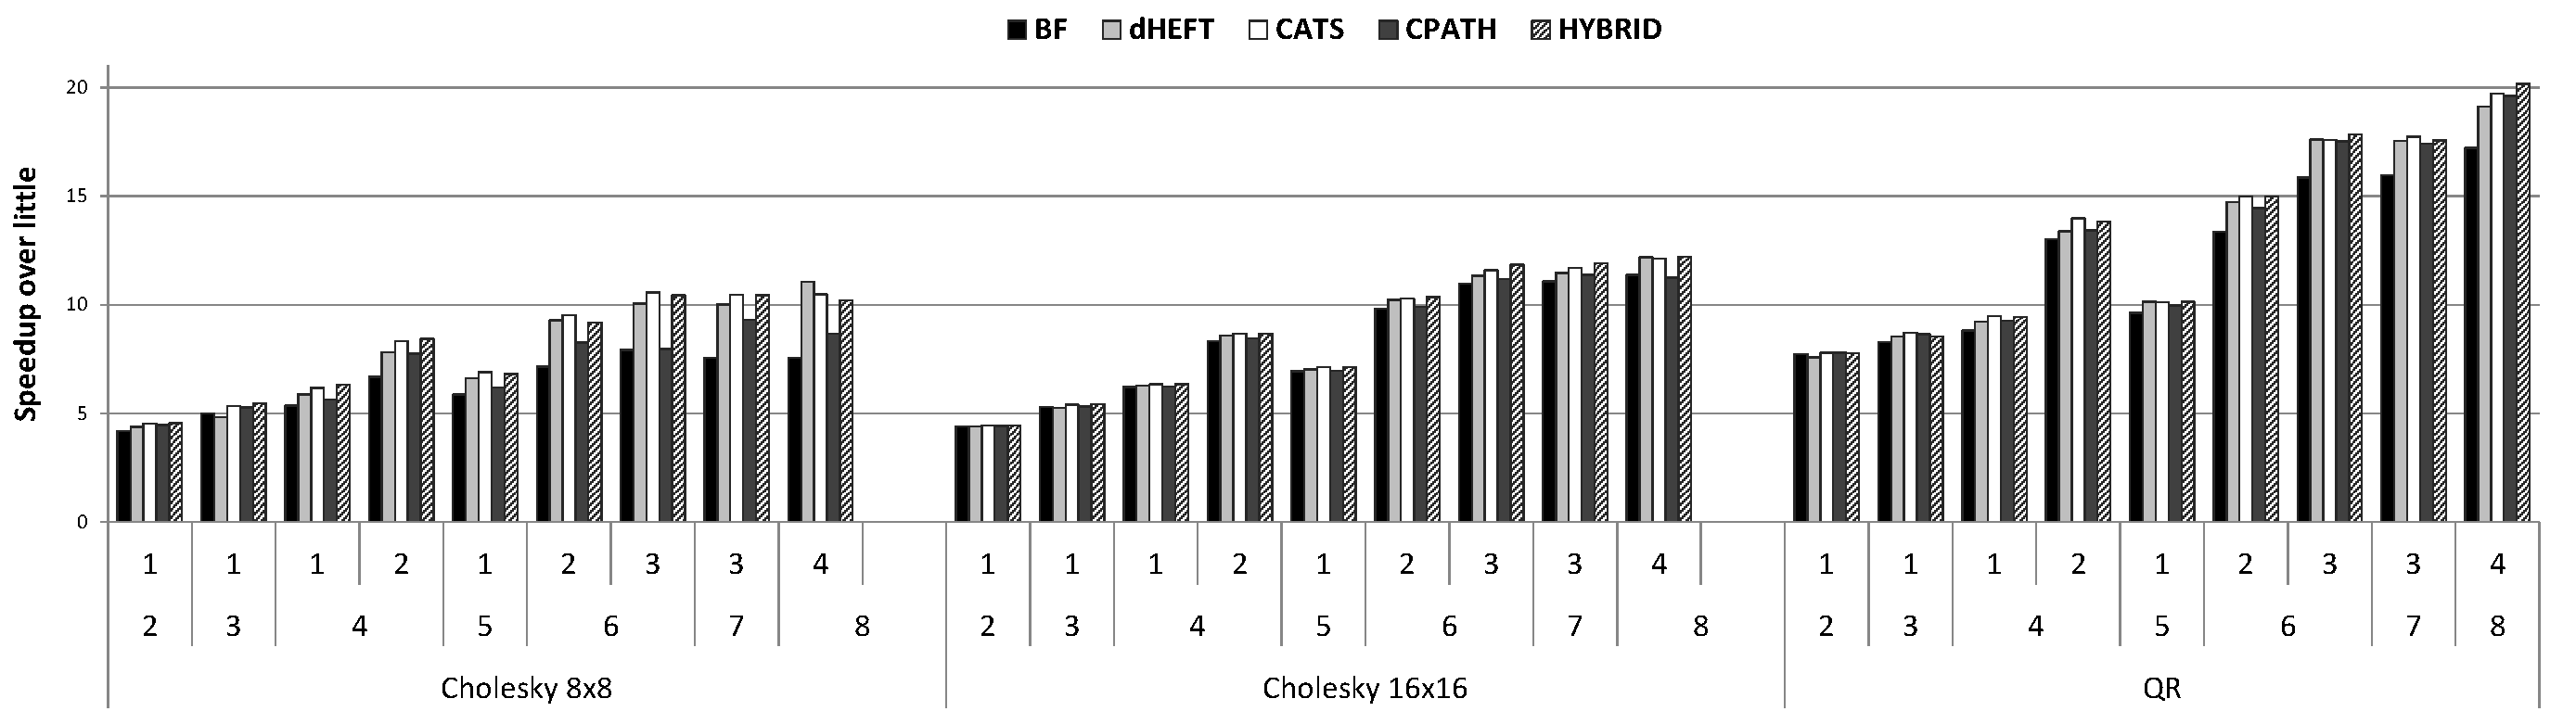
\includegraphics[width=\textwidth]{images/speedup_apps1.pdf}
	\vspace{-0.4cm}
	
	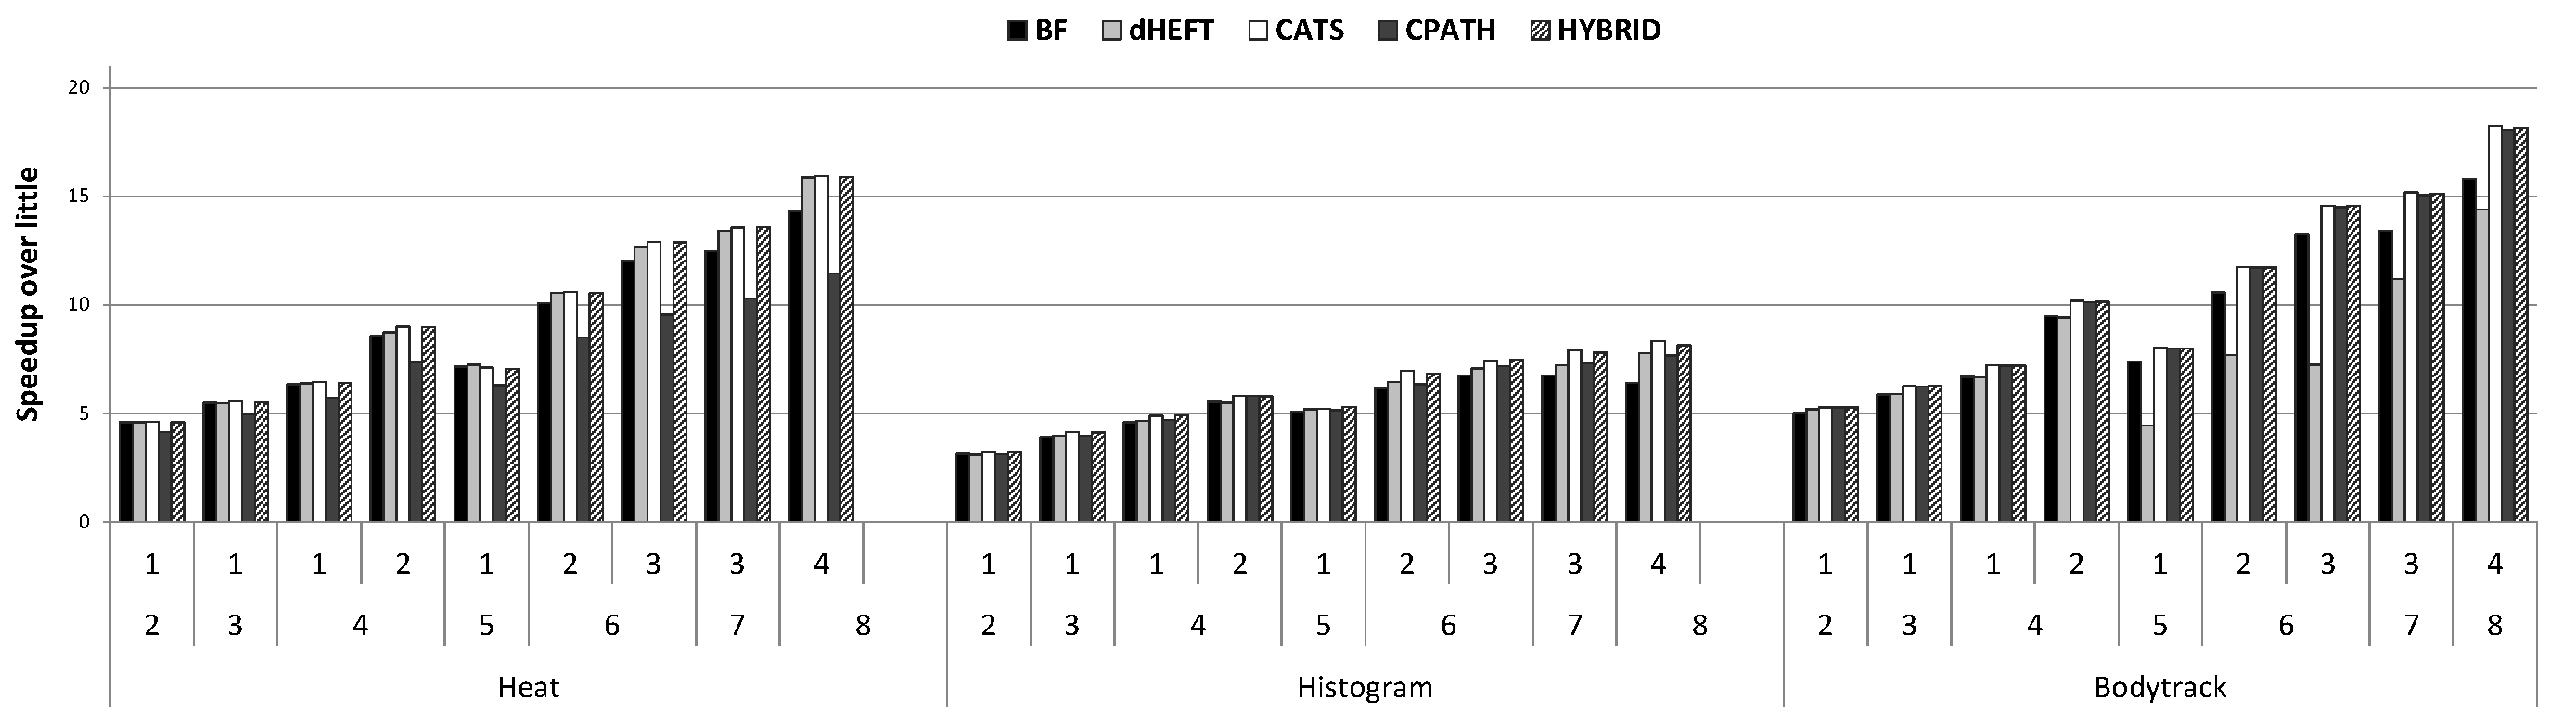
\includegraphics[width=\textwidth]{images/speedup_apps2.pdf}
	\caption{Speedups obtained for each scheduler and each application}
	\label{speedup}
	\vspace{-0.4cm}
\end{figure*}  

%--------- SUMMARY ---------------

This section showed a straight comparison between different heterogeneous schedulers.
It is important to note that schedulers like CPATH and HYBRID, that detect the time-based critical path, are the best choices when the application has a large amount of tasks.
This is because the additional overheads of these schedulers for critical path computation take place only when there are new tasks on the TDG or when there is a task exit of an untracked tt-is. 
When the TDG has been completely created, and as soon as the cost of every tt-is of the application has been tracked, the schedules of these approaches are purely beneficial.
On the other hand, schedulers like dHEFT perform the same steps for every single task that becomes ready, affecting the entire execution since the exit of a task triggers the execution of its successors that become ready. 
Thus, as the number of tasks is increased, the additional scheduling overheads are increased when using dHEFT-like approaches.
CATS scheduler is an efficient scheduling solution for any number of tasks and task cost distributions.
The additional CATS overheads take place only during task creation and are smaller than CPATH overheads with the drawback of not considering the task execution time.
If we have to choose the best and most generic heterogeneous scheduling approach among the presented schedulers the HYBRID scheduler is the best choice, since it computes an accurate critical path only when it comes at a low cost.


\subsection{Simulations}
To estimate the impact of the heterogeneity-aware schedulers on larger systems, we run three benchmarks using the TaskSim simulator~\cite{AbstrLevels_TACO12}.
The results contain a fixed scheduling overhead for all configurations, regardless of the dynamic overheads during execution (e.g., work stealing).
We simulate Cholesky, QR and Heat diffusion.
These applications feature different levels of task cost variability and have a proper amount of tasks so that the error introduced by the static overhead assumption remains negligible (e.g., bodytrack that creates 408\,525 tasks should not be compared to a 5\,000 task benchmark and static overhead).
For Cholesky, we use an input matrix of 16384$\times$16384 floats creating 512$\times$512 blocks, which results in a 32$\times$32 blocked matrix. This is because the other Cholesky configurations do not scale to 32 cores due to the limited task number. However, the task cost variability is similar to the 16$\times$ 16 input since the task size is not modified. Integral Histogram is excluded from the simulated evaluation because it does not scale beyond 16 cores.

Figures~\ref{cholesky_ts}, \ref{qr_ts} and \ref{heat_ts} show the improvement of dHEFT, CATS, HYBRID and CPATH over BF in systems with 16 and 32 cores for Cholesky, QR and heat respectively. In these experiments, the performance ratio between fast and slow cores is set to 4.5, which is the average performance ratio among the benchmarks. The heterogeneous schedulers utilize fast cores more effectively than BF, which results in larger improvements with higher number of fast cores. 

Figure~\ref{cholesky_ts} shows the improvement of the schedulers over the baseline for Cholesky. The improvement for 16 cores is comparatively small. This is due to the increased problem size used in this experiment.
This benchmark creates a small amount of critical tasks in the 32$\times$32 input, which makes the workload less sensitive to critical tasks and limits the improvement of CATS and HYBRID to a maximum of 17\%, while CPATH and dHEFT outperform BF by up to 10\%. 

%\begin{figure*}[!t]
%\begin{subfigure}[b]{0.33\textwidth}
%  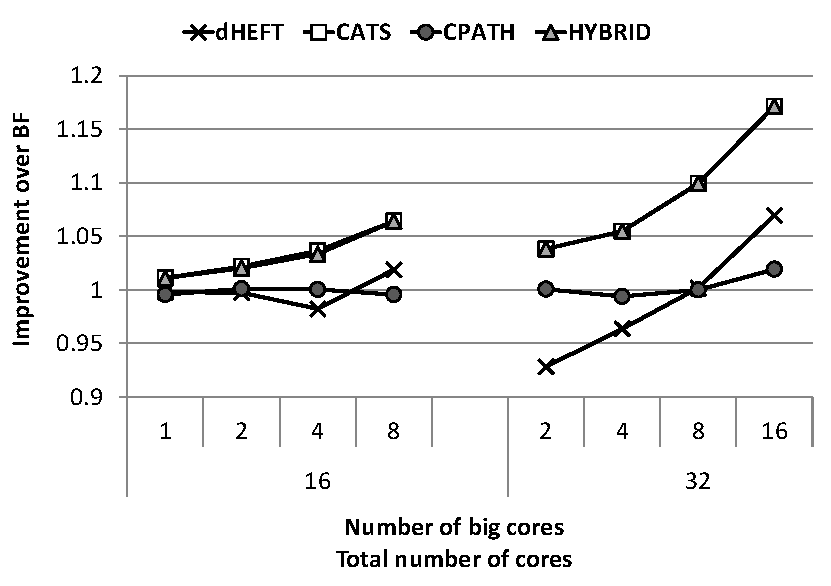
\includegraphics[width=\textwidth]{images/cholesky_TS_tall.pdf}
%  \caption{Cholesky 32$\times$32}
%  \label{cholesky_ts}
%    \vspace{-0.2cm}
%\end{subfigure}
%\begin{subfigure}[b]{0.33\textwidth}
%  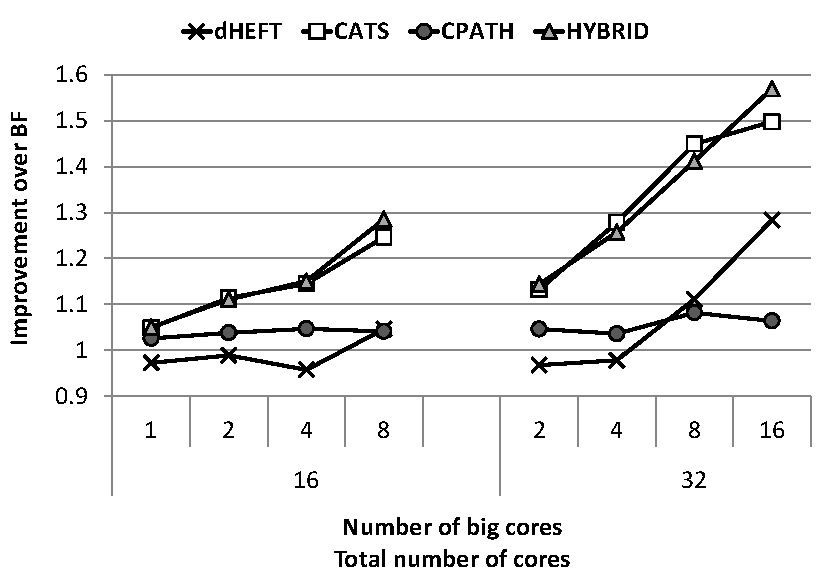
\includegraphics[width=\textwidth]{images/QR_TS_tall.pdf}
%  \caption{QR}
%  \label{qr_ts}
%    \vspace{-0.2cm}
%\end{subfigure}
%\begin{subfigure}[b]{0.33\textwidth}
%  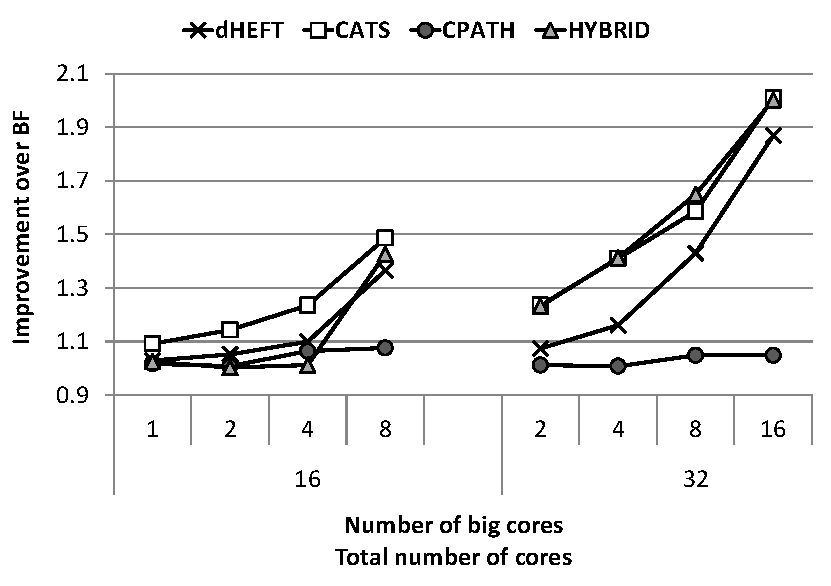
\includegraphics[width=\textwidth]{images/heat_TS_tall.pdf}
%  \caption{Heat diffusion}
%  \label{heat_ts}
%  \vspace{-0.2cm}
%\end{subfigure}  
%\caption{Improvement of heterogeneous schedulers over BF for simulated 16 and 32 core heterogeneous systems}
%\vspace{-0.5cm}
%\end{figure*}

\begin{figure}[!t]
	\centering
	\subfloat[Cholesky 32$\times$32]{
  		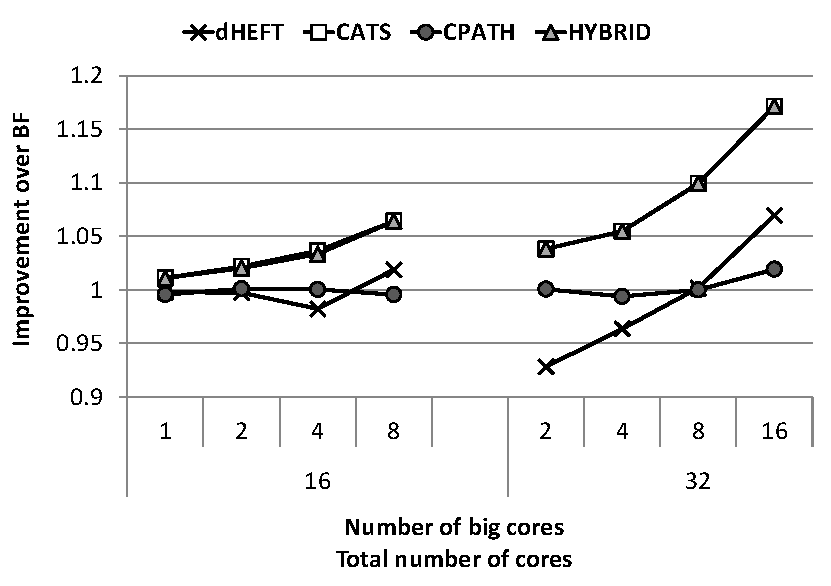
\includegraphics[width=0.65\textwidth]{images/cholesky_TS_tall.pdf}
  		\label{cholesky_ts}
	}
\\
%    \vspace{-0.2cm}
	\subfloat[QR]{
  		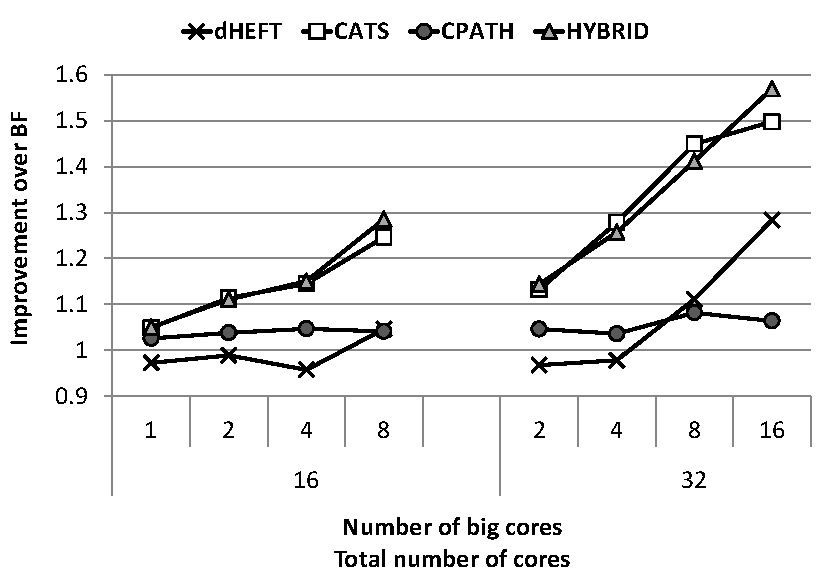
\includegraphics[width=0.65\textwidth]{images/QR_TS_tall.pdf}
  		\label{qr_ts}
  	}
\\
    %\vspace{-0.2cm}
	\subfloat[Heat diffusion]{
  		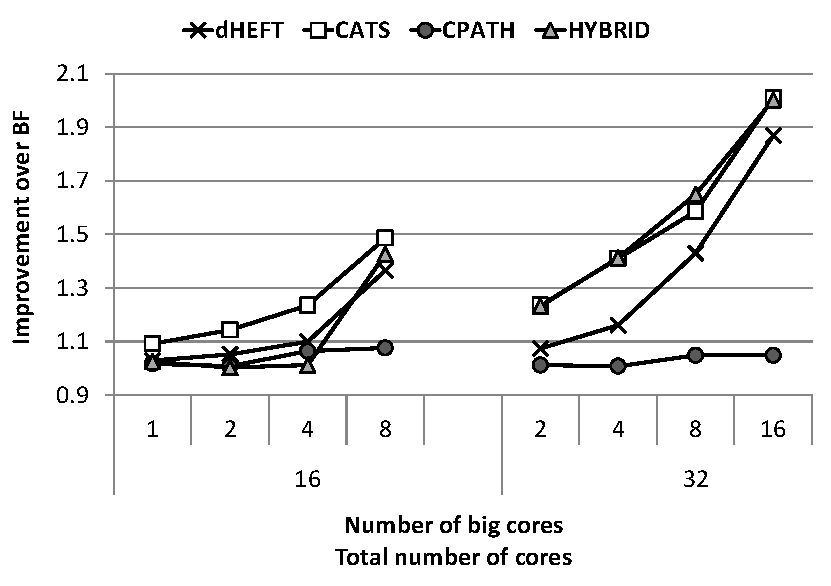
\includegraphics[width=0.65\textwidth]{images/heat_TS_tall.pdf}
  		\label{heat_ts}
  	}
%  \vspace{-0.2cm}
	\caption{Improvement of heterogeneous schedulers over BF for simulated 16 and 32 core heterogeneous systems}
%\vspace{-0.5cm}
\end{figure}

Figure~\ref{qr_ts} shows that the best option for QR, the application with the highest task cost variability, on systems with 16 or 32 cores is the HYBRID scheduler, as was also shown in the real platform evaluation, bringing improvements of 30 and 56\%.
CATS also performs well but CPATH falls short in detecting an appropriate amount of critical tasks which makes the little cores overloaded and the big cores waste their resources in work stealing.

For heat diffusion, Figure~\ref{heat_ts} shows that CATS achieves the best results outperforming BF by a factor of 2$\times$. Moreover, HYBRID achieves similar results as it performs similar schedules as CATS. However, CPATH fails to achieve optimal results because it overloads the big cores during the learning phase while the little cores remain under-utilized.


%Depending on the system and according to the application, the optimal solution for this can be found and utilize such systems effectively.


%%%%%%%%%%%%%%%%%%%%
%%%%%%%%%%%%%%%%%%%%
%\section{Related Work}
%\label{sec:related}
%The search for efficient task scheduling on multi-core systems has been intensively studied. Most scheduling heuristics target homogeneous multiprocessors, nevertheless there is an important number of studies in heterogeneous multiprocessors. In this section we give an overview of different categories of heterogeneous schedulers
% for heterogeneous systems
%, we explain some details about schedulers targeting specific systems using compute accelerators 
and explain details of previous works on criticality-aware schedulers.

%\textit{Schedulers for Heterogeneous Systems}
\textbf{Schedulers for Heterogeneous Systems: }
There are previous works on schedulers for heterogeneous systems that form four different types of schedulers: listing, clustering, guided-random, and duplication-based schedulers.

%do not consider the criticality of tasks~\cite{Hetero95, Dyn05, Gen07,Chemical, HEFT, Dup09}. These heuristics

Listing schedulers~\cite{List, DCPS, LDCP, HEFT, CrPathDup, Li2,Li5} have two scheduling stages. In the first stage, each task is given a priority based on the policy defined in each algorithm. In the second stage, tasks are assigned to processors depending on their priorities. Most criticality-aware schedulers fall in this category, and we discuss them in Section~\ref{sec.relwork_critical}. The scheduler proposed in this paper is also a list scheduler.

Clustering schedulers~\cite{Hypertool, DSC, DCPS, Hetero95} first separate tasks into clusters, where each cluster is to be executed on the same processor. During the clustering stage, the algorithm assumes an unlimited number of available processors in the system. If the number of clusters exceeds the number of available cores, the \textit{merging} stage joins multiple clusters so that they match the number of available processors. An example is the Levelized Min Time~\cite{Hetero95} clustering scheduler. This heuristic clusters tasks that can execute in parallel according to their \textit{level} (i.e. sibling nodes in a graph have the same level), and assigns priorities to the tasks in a cluster according to their cost, (i.e. tasks with the highest cost have the highest priority). The task-to processor assignment is done in decreasing order of priority.

Guided-random schedulers randomize their schedules by applying policies influenced by other sciences. Genetic algorithms~\cite{Gen07} group tasks into generations and schedule them according to a randomized genetic technique. Chemical reaction algorithms~\cite{Chemical, LiChemical} mimic molecular interactions to map tasks to processors. Some of these guided-random approaches are designed for heterogeneous systems~\cite{Gen07, Chemical}. The scheduler by Page et al.~\cite{Dyn05} enables dynamic scheduling of multiple-sized tasks for heterogeneous systems, but it lacks support of inter-task dependencies.

Duplication-based schedulers~\cite{Dup03, Dup11, Dup09} aim to eliminate communication costs between processors by scheduling tasks and their successors on the same processor. If a task has many successors, it is duplicated and executed in multiple cores prior to its successors to reduce communication costs.
%all successor tasks get the data from their predecessors with the lowest communication cost. 
This scheduling may introduce redundant task duplications tasks which may lead to bad schedules. The Heterogeneous Economical Duplication scheduler~\cite{Dup09} performs task duplication cautiously as it removes the redundant duplicates if they do not affect performance. 

These previous works schedule tasks statically and assume the prior knowledge of the task execution times on the different processor types in the heterogeneous system.

\if 0
\subsection{Schedulers for Compute Accelerators}

The schedulers in the previous section target the scheduling of generic TDGs on generic heterogeneous architectures. In this section we cover schedulers that target specific systems with compute accelerators. These works are more focused on the scheduling of tasks on the target platform based on the abstractions provided by the corresponding mixture of programming models for the general-purpose processors and the compute accelerators in the system.

Most heterogeneous systems with compute accelerators nowadays combine general-purpose CPUs and GPU compute accelerators. There is a set of programming models providing abstractions to ease the development of applications on these platforms. OmpSs~\cite{OmpSs_PPL11, OmpSs} offers this abstraction by allowing multiple implementations of a given task to be executed on different processing units~\cite{Judit}. The scheduler then assigns the execution of a task to the best resource according to its earliest finish time. Another case is StarPU~\cite{starpu}, a library that offers runtime heterogeneity support and provides priority schedulers for task-to-processor allocation. AHP~\cite{AHP} is another framework that generates software pipelines for heterogeneous systems and schedules tasks to their earliest executor, based on profiling information gathered prior to runtime.

None of these works, however, take into account the criticality of tasks regarding task dependencies, but they rather focus on the earliest execution time of individual tasks on the processor types in the specific system configuration.
\fi

%\subsection{Criticality-Aware Schedulers}
\label{sec.relwork_critical}
\textbf{Criticality-Aware Schedulers: }
Several previous works propose scheduling heuristics that focus on the critical path of a TDG to reduce total execution time~\cite{DCPS, LDCP, HEFT, CrPathDup, Moschakis2015}. To identify the tasks on the critical path, most of these works use the concept of \textit{upward rank} and \textit{downward rank}. The upward rank of a task is the maximum sum of computation and communication cost of the tasks in the dependency chains from that task to an exit node in the graph. The downward rank of a task is the maximum sum of computation and communication cost of the tasks in the dependency chain from an entry node to that task. Each task has an upward rank and downward rank for each processor type in the heterogeneous system, as the computation and communication costs differ across core types.

The Heterogeneous Earliest Finish Time (HEFT) algorithm~\cite{HEFT} maintains a list of tasks sorted in decreasing order of their upward rank. At each schedule step, HEFT assigns the task with the highest upward rank to the processor that finishes the execution of the task at the earliest possible time. Another work is the Longest Dynamic Critical Path (LDCP) algorithm~\cite{LDCP}. LDCP also statically schedules first the task with the highest upward rank on every schedule step. The difference between LDCP and HEFT is that LDCP updates the computation and communication costs on multiple processors of the scheduled task by the costs discovered in the processor to which it was assigned.

The Critical-Path-on-a-Processor (CPOP) algorithm~\cite{HEFT} also maintains a list of tasks sorted in decreasing order as in HEFT, but in this case it is ordered according to the addition of their \textit{upward rank} and \textit{downward rank}. The tasks with the highest \textit{upward rank + downward rank} belong to the critical path. On each step, these tasks are statically assigned to the processor that minimizes the critical-path execution time.

%The drawback of static listing algorithms is the static priority assignment can lead to wrong schedules at runtime~\cite{DCP}. 

The main weaknesses of these works are that (a) they assume prior knowledge of the computation and communication costs of each individual task on each processor type, (b) they operate statically on the whole TDG, so they do not apply to dynamically scheduled applications where only a part of the TDG is available at any given time, and (c) most of them use synthetic TDGs that are not necessarily representative of the dependencies in real workloads.

%These algorithms assume the prior knowledge of the execution time of each task in the task dependency graph. Moreover, they use static scheduling, namely the computation of the critical path and task-to-processor allocation are decided before the execution of the program. This can lead to wrong predictions of the critical path which, in practice, changes during runtime.





%%%%%%%%%%%%%%%%%%%
%%%%%%%%%%%%%%%%%%%


\section{Conclusions}
\label{sec.scheduling.conclusions}
We introduced the first critical-path-aware dynamic scheduler for heterogeneous systems as well as the first hybrid criticality-aware scheduler. Like CATS and contrary to previous works on criticality-aware scheduling that use synthetic TDGs and require prior knowledge of profiling information, our proposals work on real platforms with real applications and do not require off-line profiling.
%, they are implementable and work without the need of profiling.

We implemented and evaluated our scheduling proposals in the runtime system of the OmpSs programming model.
We showed that even if the accuracy of CPATH is higher in terms of task criticality identification, it does not always increase performance. 
Factors like the number of tasks and task cost variability play an important role on choosing the most appropriate scheduling policy and improve the performance of task-based applications.
The implementations shown in this paper will be included in the next stable release of the OmpSs programming model. 
Furthermore, the described policies are expected to be applicable to other task-based programming models with support for task dependencies. 
%The presented schedulers assume two core types.
%by manually choosing the cores that would act as fast, which limits the scheduling effect.
%To improve this, the schedulers can be modified to assign different levels of criticality to the tasks and let the cores, according to their type, execute the tasks with the corresponding criticality level.

%After determining the critical path, the scheduler could also consider the second, third etc. longest paths and insert their tasks in the corresponding ready queues. 
%The user has to specify which cores are considered as fast for the effective execution of the critical tasks. 
%We implemented and evaluated our criticality-aware task scheduler in the runtime system of the OmpSs programming model getting satisfactory results. The implementation shown in this paper will be included in the next stable release of OmpSs. Furthermore, there are no restrictions on applying our policy to other task-based programming models with support for task dependencies. 
    
%From our experiments on a real heterogeneous multi-core platform, we found a consistent performance improvement over the default breadth-first scheduling policy and a dynamic implementation of Heterogeneous Earliest Finish Time. The improvement of our proposal, which in most cases ranges from 10 to 20\% and reaches up to 30\%, is larger as we increase the number of cores. This gives a positive projection for CATS, as it is expected that the number of cores in multi-cores will increase throughout future generation designs.

%From our simulation experiments, we found out that the improvement of CATS increases over the baseline with larger differences of performance among fast and slow cores. We explored performance ratios between two and four times faster fast cores over slow cores, with improvements ranging from 30\% to 170\%. 

In conclusion, this chapter showed the potential of different heterogeneous schedulers to speed up dependency-intensive applications and take advantage of the asymmetric compute resources.


%For future work, we aim to extend the scheduling policy to be adaptive so it can dynamically adjust its flexibility and work stealing policy depending on the application characteristics and availability of resources at runtime.

%, and dynamically adapt its configuration to the one that best fits this combination.


